\documentclass{article}

% Bibliography
\usepackage{natbib}
\bibpunct{(}{)}{;}{a}{}{;}

% Use 'It was found that A is B (Name 1234)' style
\setcitestyle{authoryear,open={},close={}}

% Affiliations
\usepackage{authblk}
\title{pirouette: Determining the error BEAST2 makes in inferring a phylogeny}
\author[1]{Rich\`el J.C. Bilderbeek}
\author[1]{Giovanni Laudanno}
\author[1]{Rampal S. Etienne}
\affil[1]{Groningen Institute for Evolutionary Life Sciences, University of Groningen, Groningen, The Netherlands}

% Use double spacing
\usepackage{setspace}
\doublespacing

\usepackage{listings}
\usepackage{hyperref}
\usepackage{todonotes}
\usepackage{verbatim}
\usepackage{pgf}
\usepackage{bm}
\usepackage{multirow}
\usepackage{amsfonts}
\usepackage{array}
\usepackage{array}
\usepackage{booktabs}
\newcolumntype{C}[1]{>{\centering\arraybackslash}p{#1}}
\newcolumntype{L}[1]{>{\raggedright\arraybackslash}p{#1}}
\usepackage{longtable}

% sidewaysfigure
\usepackage{rotating}

% Style of listings
% From http://r.789695.n4.nabble.com/How-to-nicely-display-R-code-with-the-LaTeX-package-listings-tp4648110.html
\usepackage{fancyvrb} 
\definecolor{codegreen}{rgb}{0,0.6,0}
\definecolor{codegray}{rgb}{0.5,0.5,0.5}
\definecolor{codepurple}{rgb}{0.58,0,0.82}
\definecolor{backcolor}{rgb}{0.95,0.95,0.92}
\lstdefinestyle{mystyle}{
  language=R,% set programming language
  basicstyle=\ttfamily\small,% basic font style
  commentstyle=\color{gray},% comment style
  % numbers=left,% display line numbers on the left side
  numberstyle=\scriptsize,% use small line numbers
  numbersep=10pt,% space between line numbers and code
  tabsize=2,% sizes of tabs
  showstringspaces=false,% do not replace spaces in strings by a certain character
  captionpos=b,% positioning of the caption below
  breaklines=true,% automatic line breaking
  escapeinside={(*}{*)},% escaping to LaTeX
  fancyvrb=true,% verbatim code is typset by listings
  extendedchars=false,% prohibit extended chars (chars of codes 128--255)
  alsoletter={.<-},% becomes a letter
  alsoother={$},% becomes other
  otherkeywords={!=, ~, $, \&, \%/\%, \%*\%, \%\%, <-, <<-, /},% other keywords
  deletekeywords={c}% remove keywords 
}
\lstset{style=mystyle}

% Adds numbered lines
\usepackage{lineno}
\linenumbers

% Rename 'Abstract' to 'Summary 
\usepackage[english]{babel}
\addto{\captionsenglish}{\renewcommand{\abstractname}{Summary}}

%comments
\newcommand{\giovanni}[1]{\textcolor{blue}{\textbf{[GL: #1]}}}
\newcommand{\richel}[1]{\textcolor{orange}{\textbf{[RB: #1]}}}
\newcommand{\rampal}[1]{\textcolor{green}{\textbf{[RSE: #1]}}}


\begin{document}

\maketitle

\begin{abstract}

  \textbf{1. }
    BEAST2 is a popular Bayesian phylogenetics software tool,
    that takes an alignment of characters (usually nucleotides) 
    and an inference model to create a
    posterior of jointly-estimated phylogenies and model parameter 
    estimates. An important ingredient of BEAST2 is 
    the model for the species tree prior, 
    and the tool can in principle be used for inference of 
    macroevolutionary processes underlying the species tree. 
    However, only models that allow for fast computation of 
    the prior probability are possible in practice. 
    This begs the question how accurate the tree estimation is 
    when the real macroevolutionary processes are different 
    from those assumed in BEAST2. \\
  \textbf{2. }
    Here we present \verb;pirouette;, 
    a free, libre and open-source R package that assesses 
    the inference error BEAST2 makes based on a known/true 
    phylogeny, for example generated by a new 
    macroevolutionary diversification model. \\
  \textbf{3. }
    We describe \verb;pirouette;'s usage and the biological scientific
    question it can answer, including full examples. \\
  \textbf{4. }
    Last, we discuss the results obtained by the examples. \\
\end{abstract}

{\bf Keywords:} computational biology, evolution, phylogenetics, BEAST2, pirouette, R

%%%%%%%%%%%%%%%%%%%%%%%%%%%%%%%%%%%%%%%%%%%%%%%%%%%%%%%%%%%%%%%%%%%%%%%%%%%%%%%%%%%%%%
\section{Introduction}
%%%%%%%%%%%%%%%%%%%%%%%%%%%%%%%%%%%%%%%%%%%%%%%%%%%%%%%%%%%%%%%%%%%%%%%%%%%%%%%%%%%%%%

The development of new powerful inference tools, 
such as BEAST [\cite{drummond2007beast}], 
MrBayes [\cite{huelsenbeck2001mrbayes}]
or RevBayes [\cite{hohna2016revbayes}], 
allows to build phylogenetic trees 
from character data (usually nucleotide sequences) extracted 
from extant (but also extinct) organisms.
This has constituted an important step forward 
in our understanding of how species evolve.
Such tools have been increasingly exploited to hypothesize 
and test what the main drivers and modes for diversification are.

Because BEAST performs a Bayesian analysis, 
it does not only need character data but also tree priors, 
describing how the diversification occurs, to return posterior phylogenies.
BEAST uses standard tree priors such as Yule or 
constant-rate birth-death [\cite{nee1994reconstructed}] models.
These models are most commonly picked in biological research,
as these are of a desired minimum biological complexity, 
yet computationally fast enough.
The recent development of BEAST2 [\cite{bouckaert2014beast}] provides, 
unlike its predecessor, the possibility for third-party users 
to use their own new or preferred diversification model, 
if an algorithm is provided to calculate the probability 
of a tree given such a diversification model.
There have been plenty of these models (and their associated probability algorithms) 
developed, among others, those in which diversification is 
time-dependent [\cite{nee1994reconstructed}, \cite{rabosky2008explosive}], 
or diversity-dependent [\cite{etienne2011diversity}],
or that can shift [\cite{etienne2012conceptual}, \cite{rabosky2014automatic}, \cite{alfaro2009nine}, the SLS model. Laudanno et al., in preparation].
Other birth-death models treat speciation as a process that takes time [\cite{rosindell2010protracted}][\cite{etienne2012prolonging}], or that happens in bursts of simultaneous events [Laudanno et al., in preparation], or that
depends on a trait that has two [\cite{maddison2007estimating}], 
or more [\cite{fitzjohn2012diversitree}] states,
or even allows concealed states [\cite{beaulieu2016detecting}] 
or a combination of all these [\cite{herrera2018detecting}].
Note all of these diversification models are available in BEAST2, 
but the option is available.

For a given phylogeny, the parameter values of the diversification model 
are usually estimated using maximum likelihood.
For such  models, 
it is a standard practice to assess their performance 
on a controlled environment: 
phylogenies are simulated with known parameters, 
and then the estimated parameters are compared with the original parameters.
If the likelihood proves to be effective to describe the process, 
it can potentially be implemented into BEAST2 as a new prior. 
However, in many cases the computation of this likelihood (the tree prior) 
is computationally demanding and it is unfeasible to use it 
in a Bayesian inference framework where it needs to be 
computed millions to billions of times.
However, if the data are very informative, the influence of the prior 
is often relatively small, and hence under this assumption 
it has become common practice to use already existing BEAST2 priors. 
However, it is unclear whether this assumption holds.
Here we introduce a pipeline to assess this assumption 
for any given diversification model. 
Briefly, it consists of the following steps: 
first simulate a phylogeny 
according to the mechanisms proposed by the new diversification model, 
then simulate a nucleotide alignment 
and use current inference tools (such as BEAST2) to estimate the phylogeny. 
If the estimated tree differs only slightly from the original phylogeny, 
the original assumption is justified and the simple diversification models 
in the inference tools suffice. 
If the trees differ markedly, it will be worth the effort and computational burden 
to develop a species tree module to be used in these tools.
Our pipeline is programmed as an R package and is called 
\verb;pirouette; it is built on \verb;babette; [Bilderbeek \& Etienne, 2018], 
which calls BEAST2 [\cite{bouckaert2014beast}]. 
With \verb;pirouette;, one
can easily measure the error made by Bayesian inference in recovering
any given phylogeny, helping us to evaluate the necessity of a new diversification model.

%%%%%%%%%%%%%%%%%%%%%%%%%%%%%%%%%%%%%%%%%%%%%%%%%%%%%%%%%%%%%%%%%%%%%%%%%%%%%%%%%%%%%%
\section{Description}
%%%%%%%%%%%%%%%%%%%%%%%%%%%%%%%%%%%%%%%%%%%%%%%%%%%%%%%%%%%%%%%%%%%%%%%%%%%%%%%%%%%%%%

\verb;pirouette; is written in the R programming language (\cite{R}).
The goal of \verb;pirouette; is to measure the inference error BEAST2
makes for a given reconstructed phylogeny, simulated under the mechanisms of a (possibly new) diversification model, which we will refer to as the 'generative prior'. Such a study will typically construct phylogenies for different combinations of the diversification model's parameters, to assess under which scenarios the error made by BEAST2 cannot be neglected. Although a well-conducted theoretical study uses many replicates, this article only shows examples with one replicate, for the sake of clarity.

\verb;pirouette; is very flexible and allows the user to specify a big variety of custom settings. These settings can be grouped in macro-sections, according to how they operate in the pipeline. We summarize them in Table~\ref{tab:definitions}.

Although many possible tests can be performed, we present here only four example research questions (ERQ) that \verb;pirouette; can answer. For these ERQs we will estimate the error made by BEAST2 when using birth-death tree prior, in recovering an original tree generated under a Yule generative prior.

\begin{table}
\centering
  \begin{tabular}{|@{}c|@{}l|p{6cm}@{}|}
    \hline
    \textbf{Name} & \textbf{Meaning} & \textbf{Definition} \\ 
    \hline
    $\mathit{t}$ & tree prior & Used to simulate a DNA alignment\\
    $\mathit{c}$ & clock model & Specifies the clock for the DNA mutation rates\\
    $\mathit{s}$ & site model & Specifies the nucleotide substitution model\\
    $\mathit{\mu}$ & mutation rate & Defines the pace at which mutation occurs\\
    $\mathit{r}$ & root sequence & Specifies DNA sequence at the root of the tree\\
    $\mathit{m}$ & MRCA prior & Prior knowledge of a most recent common ancestor\\
    $\mathit{v}$ & MCMC settings & Setup of the Markov Chain Monte Carlo algorithm\\
    \hline
    $\mathit{P}$ & Generative prior & Specifies the diversification model according to which the 'true' tree is simulated\\
    $\mathit{A}$ & Alignment model & Model for the alignment simulation. It's a choice of
    $(\mathit{r},\mathit{\mu},\mathit{c},\mathit{s})$\\
    $\mathit{G}$ & Generative model & A combination of the chosen $(\mathit{P},\mathit{A})$\\
    $\mathit{I}$ & Inference model & Specifies how to execute the inference. It's a choice of
    $(\mathit{c},\mathit{s},\mathit{t},\mathit{m},\mathit{v})$\\
    $\mathit{C}$ & Inference conditions & Specifies under which conditions an inference model is used\\
    $\mathit{X}$ & Experiment & A combination of the chosen $(\mathit{I},\mathit{C})$\\
    $\mathit{E}$ & Error parameters & Sets how to measure errors\\
    $\mathit{T}$ & Twinning parameters & Specifies how to twin the 'true' tree\\
    \hline
  \end{tabular}
  \caption{
    Definitions of terms and relative symbols used in this article.
  }
  \label{tab:definitions}
  \giovanni{It would be nice to specify (in the first part of the table) the basic elements composing all the elements of the second part of the table. This could be probably done for "Alignment parameters", "Inference conditions" and "Twinning parameters".}
  \giovanni{Shall we add another column with the possible option for each lower case setting? e.g. "clock model" = c("strict", "rln"); "tree prior" = c("yule", "bd")}
  \giovanni{How do we specify what constitutes 'twinning parameters'?}
\end{table}

\iffalse
Experiment & Combination of an inference model and the \\ 
    & conditions to actually use it in inference \\
    Generative model & Combination of site model, clock model and \\
    & tree prior, used to simulate a DNA alignment \\
    Inference model & Combination of site model, clock model, tree prior,\\
    & MRCA prior and MCMC, used to infer \\
    & a BEAST2 posterior \\
    MCMC & Setup of the Markov Chain Monte Carlo algorithm \\
    MRCA prior & Prior knowledge of a most recent common ancestor \\
    Site model & Model for the DNA nucleotide substitions \\
    Tree prior & Model for the macroevolutionary speciation process \\
\fi

\iffalse
$\mathit{t}$ & tree prior & Used to simulate a DNA alignment\\
    $\mathit{c}$ & clock model & Specifies the clock for the DNA \\
    & & mutation rates\\
    $\mathit{s}$ & site model & Specifies how nucleotides change\\
    & & in one another\\
    $\mathit{m}$ & MRCA prior & Prior knowledge of a most recent\\
    & & common ancestor\\
    $\mathit{v}$ & MCMC settings & Setup of the Markov Chain\\
    & &  Monte Carlo algorithm\\
    
    $\mathit{G}$ & Generative model & Specifies how to create the 'true'\\
    & &  tree. It's a choice of $(\mathit{c},\mathit{s},\mathit{t})$\\
    $\mathit{T}$ & Twinning parameters & Specifies how to twin the 'true' tree\\
    $\mathit{A}$ & Alignment parameters & Parameters for the alignment\\
    & & simulation\\
    $\mathit{I}$ & Inference model & Specifies how to execute the inference. \\
    & & It's a choice of
    $(\mathit{c},\mathit{s},\mathit{t},\mathit{m},\mathit{v})$\\
    $\mathit{C}$ & Inference conditions & Specifies under which conditions an\\
    & & inference model is used\\
    $\mathit{X}$ & Experiment & A combination of the chosen $(\mathit{I},\mathit{C})$\\
    $\mathit{E}$ & Error parameters & Sets how to measure errors\\
\fi

\iffalse
\richel{
  I do think this is a clumsy paragraph. I hope you can merge it in the text
}
To explain how \verb;pirouette; measures the inference error BEAST2 makes, we first give two definitions (see Table~\ref{tab:definitions} for an overview of definitions): (1) a generative model is a combination of a known tree prior (that generated a given phylogeny) and a site and clock model (that generate an alignment from the given tree), (2) an inference model is a combination of site model, clock model, tree prior, an optional most recent common-ancestor (MRCA) prior (to create a time-calibrated phylogeny) and a Markov chain Monte Carlo (MCMC) setup.
A generative model is a known/true model underlying a phylogeny and is used to simulate DNA alignments. An inference model is used to produce a posterior distribution of trees and model parameters.
\fi

\subsection{pirouette's pipeline}

\begin{figure}
  \centering
  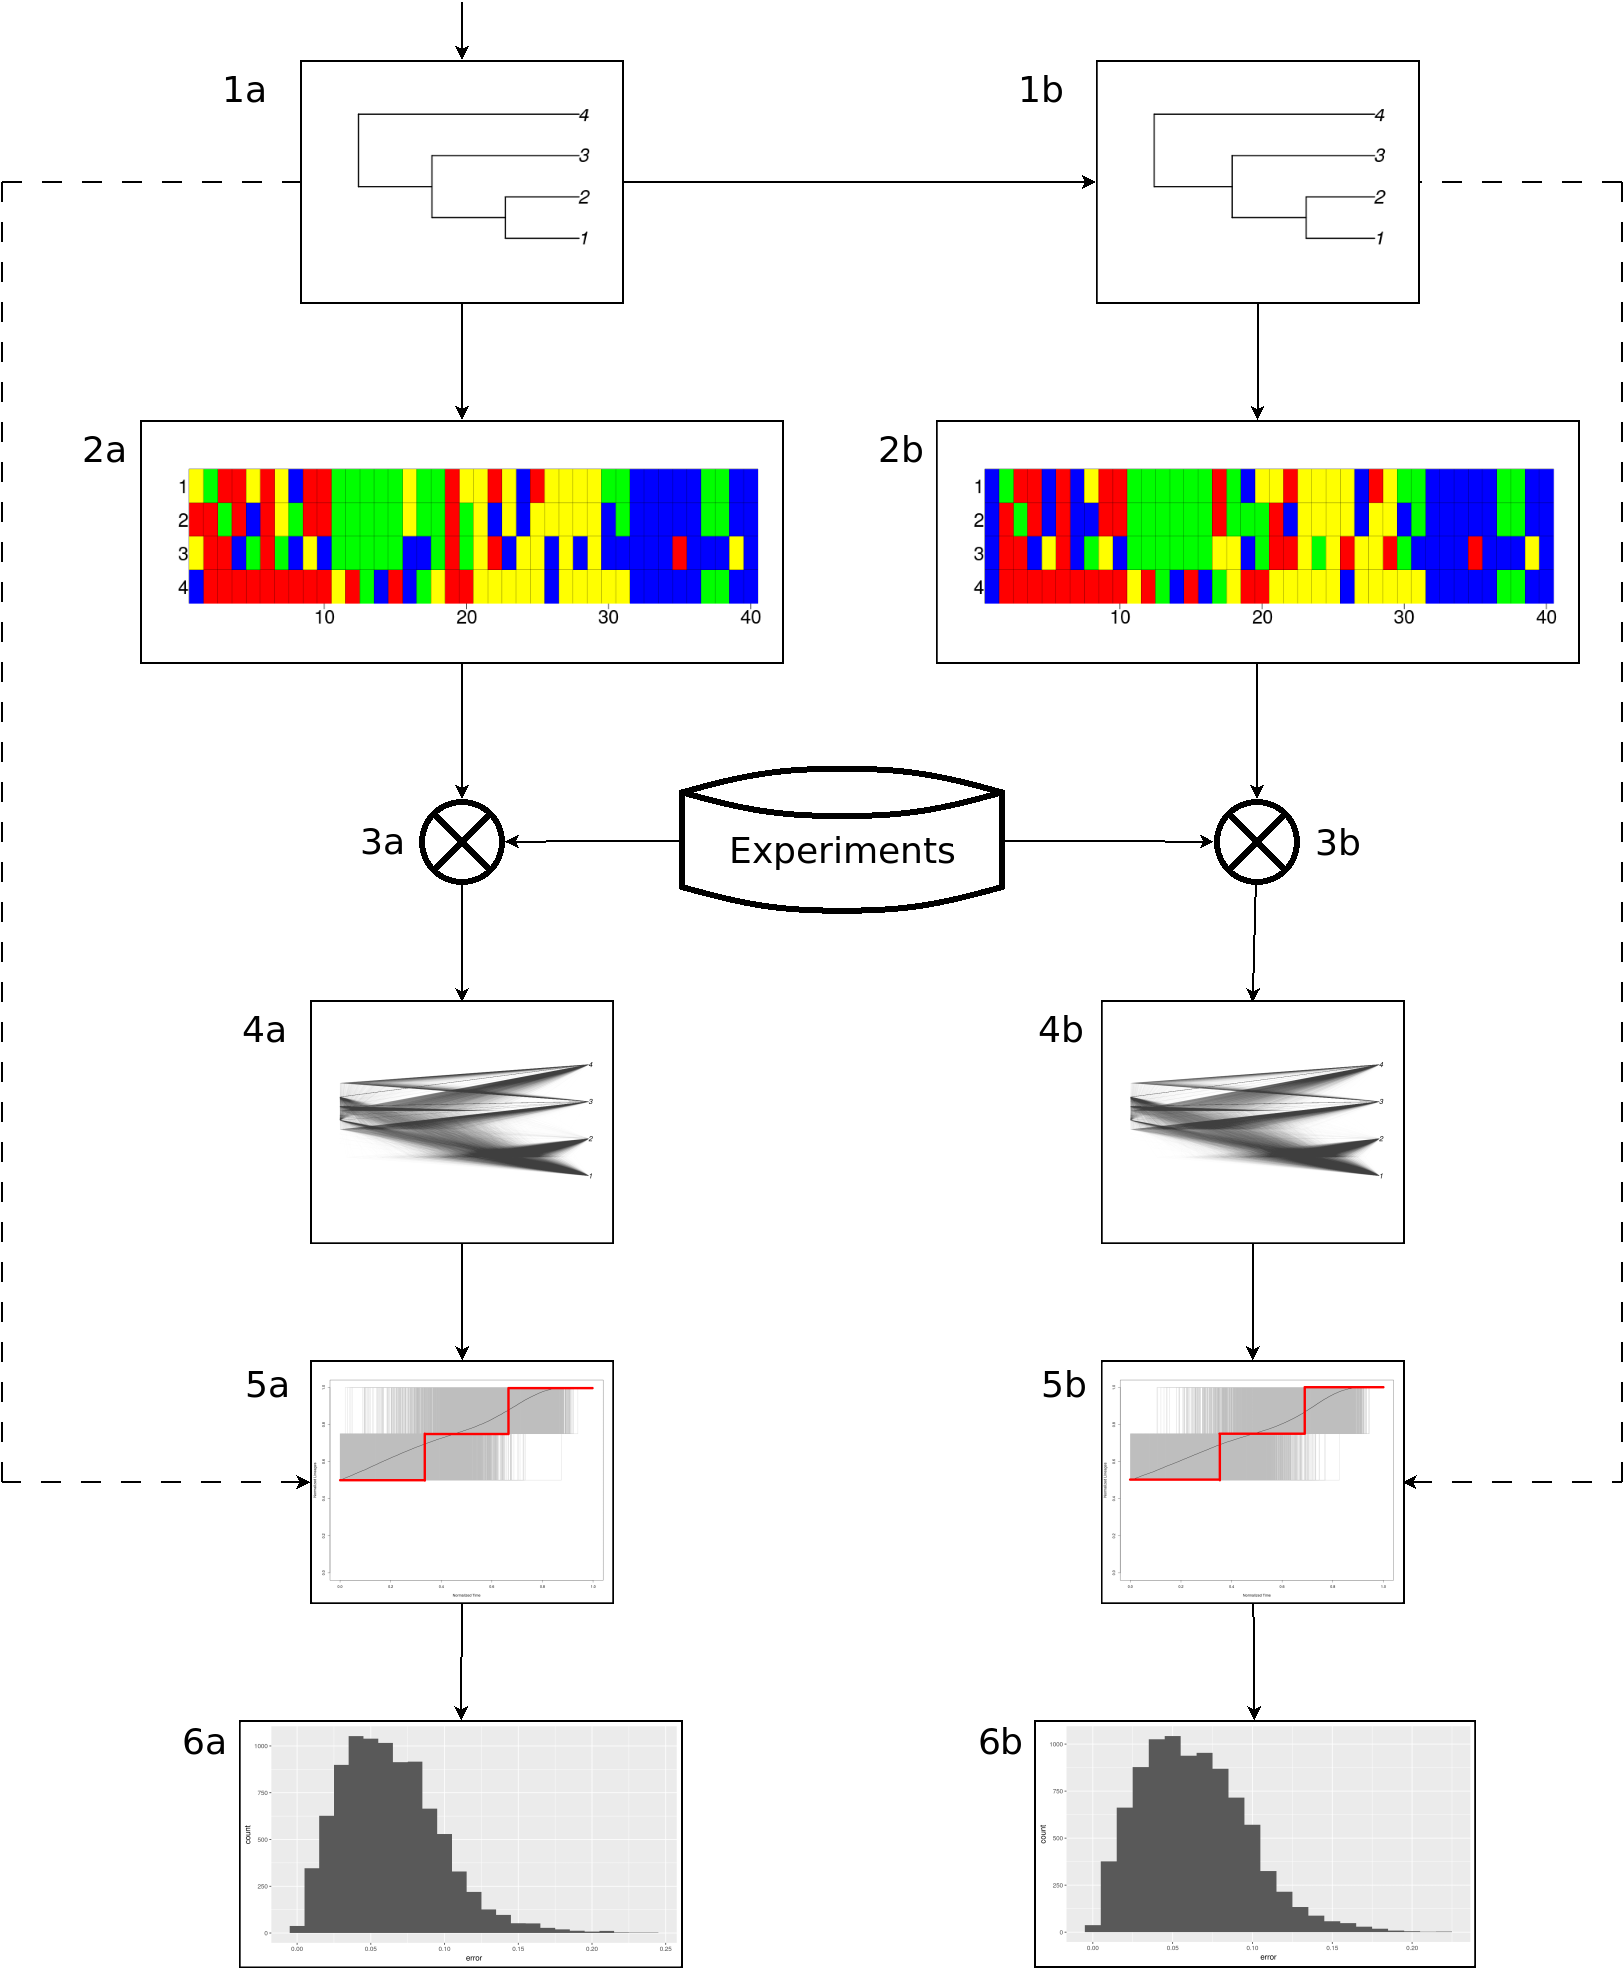
\includegraphics[width=\textwidth]{workflow.png}
  \caption{
    \texttt{pirouette} pipeline. 
    The pipeline starts from a true phylogeny (1a), that is converted to an alignment (2a). The user supplies one or more experiments. Every experiment is
    defined as a combination of an inference model and the conditions in which it is actually used in the inference. Based on the experiments and possibly the alignment (2a), experiments are selected to be actually used used in the next step (3a).
    Selected experiments use the alignment (2a) and their inference model 
    to create a BEAST2 posterior of (parameter estimates and) phylogenies (4a). The posterior trees are compared to the true phylogeny (1a) using the nLTT statistic [\cite{janzen2015approximate}]. (5a) shows the nLTT of the true tree in red,
    the nLTT of all individual posterior trees in grey, and the average nLTT statistic of all posterior trees in black. Taking the differences between the true tree's nLTT and each posterior's nLTT results in an error distribution, here displayed as a histogram
    of error values (6a). Optionally, a twin phylogeny (1b) can be generated from a true
    phylogeny (1a), which then results in an error distribution (6b) with similar intermediate steps.
  }
  \label{fig:pipeline}
    \giovanni{The black line for the average of all posterior trees is barely visible. Please, make it thicker.}
    \giovanni{Modify the figure to include elements in table~\ref{tab:definitions}. It should be specified clearly where elements corresponding to capital symbols play their roles in the pipeline. Then we should include also these elements in the caption.}
\end{figure}

\iffalse
\caption{
    \texttt{pirouette} pipeline. 
    The pipeline starts from a true phylogeny (1a), that is converted to an alignment (2a). The user supplies one or more experiments. Every experiment is
    defined as a combination of an inference model and the conditions in which it is actually used in the inference. Based on the experiments and possibly the alignment (2a), experiments are selected to be actually used used in the next step (3a).
    Selected experiments use the alignment (2a) and their inference model 
    to create a BEAST2 posterior of (parameter estimates and) phylogenies (4a). The posterior trees are compared to the true phylogeny (1a) using the nLTT statistic [\cite{janzen2015approximate}]. (5a) shows the nLTT of the true tree in red,
    the nLTT of all individual posterior trees in grey, and the average nLTT statistic of all posterior trees in black. Taking the differences between the true tree's nLTT and each posterior's nLTT results in an error distribution, here displayed as a histogram
    of error values (6a). Optionally, a twin phylogeny (1b) can be generated from a true
    phylogeny (1a), which then results in an error distribution (6b) with similar intermediate steps.
  }
\fi

The pipeline is summarized by the following steps, which will be described in detail below:
\begin{enumerate}
    \item for a given phylogeny an alignment is simulated under a known alignment model;
    \item for this alignment, according to the specified inference conditions, an inference model is picked (which may be different from the generative alignment model);
    \item the alignment is then used as BEAST2 input to infer a posterior distribution of phylogenies;
    \item posterior phylogenies are compared with the given original phylogeny to estimate the error made, according to the error parameters specified by the user;
\end{enumerate}
The pipeline is visualized in Fig.~\ref{fig:pipeline}. There is also the option to generate a 'twin tree', that goes through the same pipeline. 
The utility of this twin tree will be explained below.

The first step simulates a DNA alignment from a given 
phylogeny (Fig.~\ref{fig:pipeline}, 1a $\rightarrow$ 2a).
This operation is performed according to the alignment model specified by the user, which consists in a root DNA sequence, a DNA mutation rate, a site model and a clock model. Since all the branches must evolve at the same pace, the clock model is always set to strict for this step. \giovanni{I think we need to specify the clock model, even though the user cannot change it. This is necessary because we refer to it when specifying what it means to set the inference model equal to the generative model. Please check if my description of why the clock can only be strict is accurate.}
This step is relatively fast, but longer DNA alignments will noticeably slow down the inference step.

The second step (Fig.~\ref{fig:pipeline}, 2a $\rightarrow$ 3a)
starts from experiments as set up by the user. 
We define an experiment as the combination of an inference model 
and the conditions to actually use it in the inference step.
The inference model can be selected in two ways, either using the
generative model or selecting one or more candidates out of a list of candidate inference models.
An experiment can use the generative model as the inference model, if the generative model is known.
An experiment uses a candidate model if either the generative model is unknown,
or there is an interest in seeing how well non-generative models compete with
the generative model.
Typically, a generative model and/or a best candidate model are used in the actual inference.
When using an experiment with a generative model,
it must use the same site and clock model used in the alignment simulation,
as well as the tree prior that underlied the creation of the given phylogeny \giovanni{the tree prior appears not to be part of the alignment model. This means that should be part of the generative prior. Is it true? In case we can refer explicitly to it, according to our definitions in table \ref{tab:definitions}}. 
When using experiments with candidate models,
\verb;pirouette; selects the best candidate based
on the evidence (i.e. marginal likelihood) for the model given the alignment.
The evidence of an inference model is estimated using a nested sampling (NS)
approach, as described in \cite{maturana2018model}. The nested sampling is
performed by \verb;mcbette; [\cite{mcbette}], that calls the 'NS' BEAST2 package. 
Using BEAST2 packages (in a scripted way) can only be done under Linux and Mac,
therefore the selection of candidate models is not available directly on Windows. 
However, even on Windows systems there is the option to perform the model selection from browser, using \verb;mcbette;, yet the computation for this model selection is
restricted to one hour for free users of the host (Travis CI) continuous
integration service.

The third step infers the actual Bayesian posteriors from the simulated 
alignment (Fig.~\ref{fig:pipeline}, 2a $\rightarrow$ 3a $\rightarrow$ 4a),
using the inference models from the experiments selected in the previous step. For each selected experiment, one BEAST2 posterior is inferred, using the \verb;babette; [\cite{bilderbeek2018babette}] R package.

The fourth step compares the true tree to each posterior tree, calculating the
error using the nLTT statistic (\cite{janzen2015approximate}) 
(Fig.~\ref{fig:pipeline}, 4a $\rightarrow$ 5a), resulting
in an error distribution (Fig.~\ref{fig:pipeline}, 5a $\rightarrow$ 6a).
The nLTT statistic is used by default, but also a user-defined error statistic can be used. 
As an example, \verb;pirouette; supplies one custom error statistic,
that uses an absolute difference in the gamma statistic [\cite{pybus2000testing}].
Additionally, the user can specify the proportion of posterior phylogenies to 
discard (i.e. the burn-in), throwing away the first $10\%$
of all phylogenies by default. This burn-in is used to discard
the part of the MCMC chain that has not yet converged to a
representative part of the state space.

\subsection{Twin tree}

An optional step is to generate a 'twin tree' 
(Fig.~\ref{fig:pipeline}, 1a $\rightarrow$ 1b),
that will be analyzed in the same way as the true tree.
The twin tree has the same topology as the given phylogeny, 
yet its branching times are simulated according to 
a birth-death tree model.
\richel{Should be switched to BD, pirouette Issue 161}.
The goal of this procedure is to generate a tree
accordingly to the tree prior used in the generative model, 
that is used as a control for the main experiment.
To produce such a birth-death tree, we maximize a birth-death likelihood [\cite{nee1994reconstructed}], conditioned on having the same number of tips as the original tree, to infer its parameters.
We use these parameters, which are the per-species speciation and extinction rates, to simulate the branching times for the twin tree, which we combine with the original tree's topology. 

%%%%%%%%%%%%%%%%%%%%%%%%%%%%%%%%%%%%%%%%%%%%%%%%%%%%%%%%%%%%%%%%%%%%%%%%%%%%%%%%%%%%%%
\section{Installation}
%%%%%%%%%%%%%%%%%%%%%%%%%%%%%%%%%%%%%%%%%%%%%%%%%%%%%%%%%%%%%%%%%%%%%%%%%%%%%%%%%%%%%%

\verb;pirouette; can be installed easily from CRAN:
\rampal{be careful here; it is not on CRAN yet. Better to say it can be installed from GitHub and will be made available on CRAN)}
\richel{We adopted this policy (to say it's on CRAN in advance) with babette as well. Is this a hint to get pirouette on CRAN before the publication of this article :-) ?}
\begin{lstlisting}[language=R, floatplacement=H, frame=single]
install.packages("pirouette")
\end{lstlisting}

For the most up-to-date version, 
one can download and install the package from \verb;pirouette;'s GitHub repository:

\begin{lstlisting}[language=R, floatplacement=H, frame=single]
usethis::install_github("richelbilderbeek/pirouette")
\end{lstlisting}

To start using \verb;pirouette;, load its functions in the global namespace first:

\begin{lstlisting}[language=R, floatplacement=H, frame=single]
library(pirouette)
\end{lstlisting}
Because \verb;pirouette; calls BEAST2, BEAST2 must be installed. 
This can be done from within R, using:

\begin{lstlisting}[language=R, floatplacement=H, frame=single]
install_beast2()
\end{lstlisting}
For the option to select inference models,
\verb;pirouette; uses the "NS" BEAST2 package [\cite{maturana2018model}].
It can be installed from within R, using:

\begin{lstlisting}[language=R, floatplacement=H, frame=single]
install_beast2_pkg("NS")
\end{lstlisting}

An overview of \verb;pirouette;'s main functions is shown in 
table \ref{tab:functions}. 
We will exploit these functions to answer our research questions in the next sections.

%%%%%%%%%%%%%%%%%%%%%%%%%%%%%%%%%%%%%%%%%%%%%%%%%%%%%%%%%%%%%%%%%%%%%%%%%%%%%%%%%%%%%%
\begin{table}[h]
\centering
\begin{tabular}{ | l | l | }
\hline
\textbf{Name} & \textbf{Description} \\
\hline
\verb;pir_run; & Run \verb;pirouette; \\
\verb;create_pir_params; & Create the \verb;pirouette; parameters \\
\hline
\verb;create_alignment_params; & Create the alignment parameters \\
\verb;create_twinning_params; & Create the twinning parameters \\
\verb;create_experiment; & Create one experiment \\
\verb;create_error_measure_params; & Create the error measurement parameters \\
\hline
\end{tabular}
\caption{pirouette's main functions}
\label{tab:functions}
\end{table}
%%%%%%%%%%%%%%%%%%%%%%%%%%%%%%%%%%%%%%%%%%%%%%%%%%%%%%%%%%%%%%%%%%%%%%%%%%%%%%%%%%%%%%

All \verb;pirouette;'s functions are documented. 
Useful examples and sensible defaults, 
which we will refer to in the next sections, 
can be accessed from the documentation.

%%%%%%%%%%%%%%%%%%%%%%%%%%%%%%%%%%%%%%%%%%%%%%%%%%%%%%%%%%%%%%%%%%%%%%%%%%%%%%%%%%%%%%
\section{Usage: Example Research Question 1}
%%%%%%%%%%%%%%%%%%%%%%%%%%%%%%%%%%%%%%%%%%%%%%%%%%%%%%%%%%%%%%%%%%%%%%%%%%%%%%%%%%%%%%

A first research question that \verb;pirouette; can answer is:

"What is the error made by BEAST2 from a phylogeny using the same diversification model as it was generated by?"

\richel{Suggest: use BD tree (again)} \giovanni{I think in this case we should indeed use a Yule tree prior, as we want to use a generative prior that is not birth-death (which is what BEAST2 is using for the inference). What do you think?}
We start from a tree simulated under a Yule (pure-birth) generative prior. We choose to use a tree with five taxa and a crown age of ten.

\begin{lstlisting}[
    language=R, floatplacement=H, frame=single, 
    label = {lst:create_yule_tree}, 
    caption = {Create a Yule tree}
  ]
phylogeny <- create_yule_tree(n_taxa = 5, crown_age = 10)
\end{lstlisting}

\begin{figure}[h]
  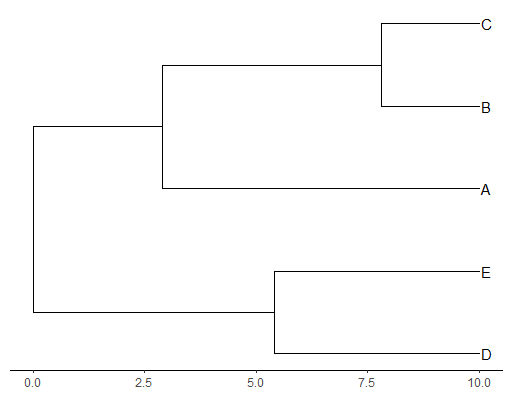
\includegraphics[width=\textwidth]{figure_bd.png}
  \caption{The Yule tree, as created by listing \ref{lst:create_yule_tree}}
\end{figure}

The first step in \verb;pirouette; is to simulate a DNA alignment from the given phylogeny. 
To do so, we must specify the DNA root sequence and a mutation rate. 
In this example, the DNA root sequence consists out of four block of 250 nucleotides each, 
where the per-nucleotide mutation rate is 0.1 mutations per unit time.

\begin{lstlisting}[
    language=R,
    floatplacement=H, frame=single,
    label = {lst:create_alignment}, 
    caption = {Create an alignment}
  ]
alignment_params <- create_alignment_params(
  root_sequence = create_blocked_dna(length = 1000),
  mutation_rate = 0.1
)
\end{lstlisting}

By default, an alignment is created using a Jukes-Cantor (JC) site model
and a strict clock model. 
A JC site model assumes that mutation rates from any nucleotide to any other 
are equal and constant. 
A strict clock model assumes that the mutation rates of all species are equal and constant.
Due to this, we state that the generative model for the alignment is
a JC site model and a strict clock model.

In the second step we state our experiments. In this context, we
define an experiment as a combination of an inference model
and the conditions under which a Bayesian inference is executed.
Within this example, we specify that our experiment uses the
generative model (which means that the inference model will be 
a combination of JC site model, strict clock model and Yule tree prior), 
will always be run and we skip to measure the evidence for our model.

\begin{table}
  \begin{tabular}{ | c | c | c | l | }
    \hline
    \textbf{model type} & \textbf{run if} & \textbf{measure evidence} & \textbf{inference model} \\ 
    \hline
    generative & always & no & JC, strict, Yule \\
    \hline
  \end{tabular}
  \caption{
    Experimental setup to answer the first research question.
    JC: Jukes-Cantor site model.
    strict: strict clock model.
    Yule: Yule (pure-birth) tree prior.
  }
  \label{tbl:RQ1}
\end{table}

Due to sensible defaults, specifying this
results in:

\begin{lstlisting}[
  language=R, 
  floatplacement=H, frame=single,
  label = {lst:create_generative_experiment},
  caption = {
    Create a default experiment, as described in Table~\ref{tbl:RQ1}.
  }
]
experiments <- list(create_experiment())
\end{lstlisting}

All the \verb;pirouette; arguments are bundled
and checked by \verb;create_pir_params;:

\begin{lstlisting}[language=R, floatplacement=H, frame=single]
pir_params <- create_pir_params(
  alignment_params = alignment_params,
  experiments = experiments
)
\end{lstlisting}

Running the experiment:

\begin{lstlisting}[language=R, floatplacement=H, frame=single]
errors <- pir_run(
  phylogeny,
  pir_params = pir_params
)
\end{lstlisting}

\verb;pirouette; has a plotting function used for convenience:

\begin{lstlisting}[language=R, floatplacement=H, frame=single]
pir_plot(errors)
\end{lstlisting}

The resulting figure is shown in figure \ref{fig:example_1}.

\begin{figure}[h]
  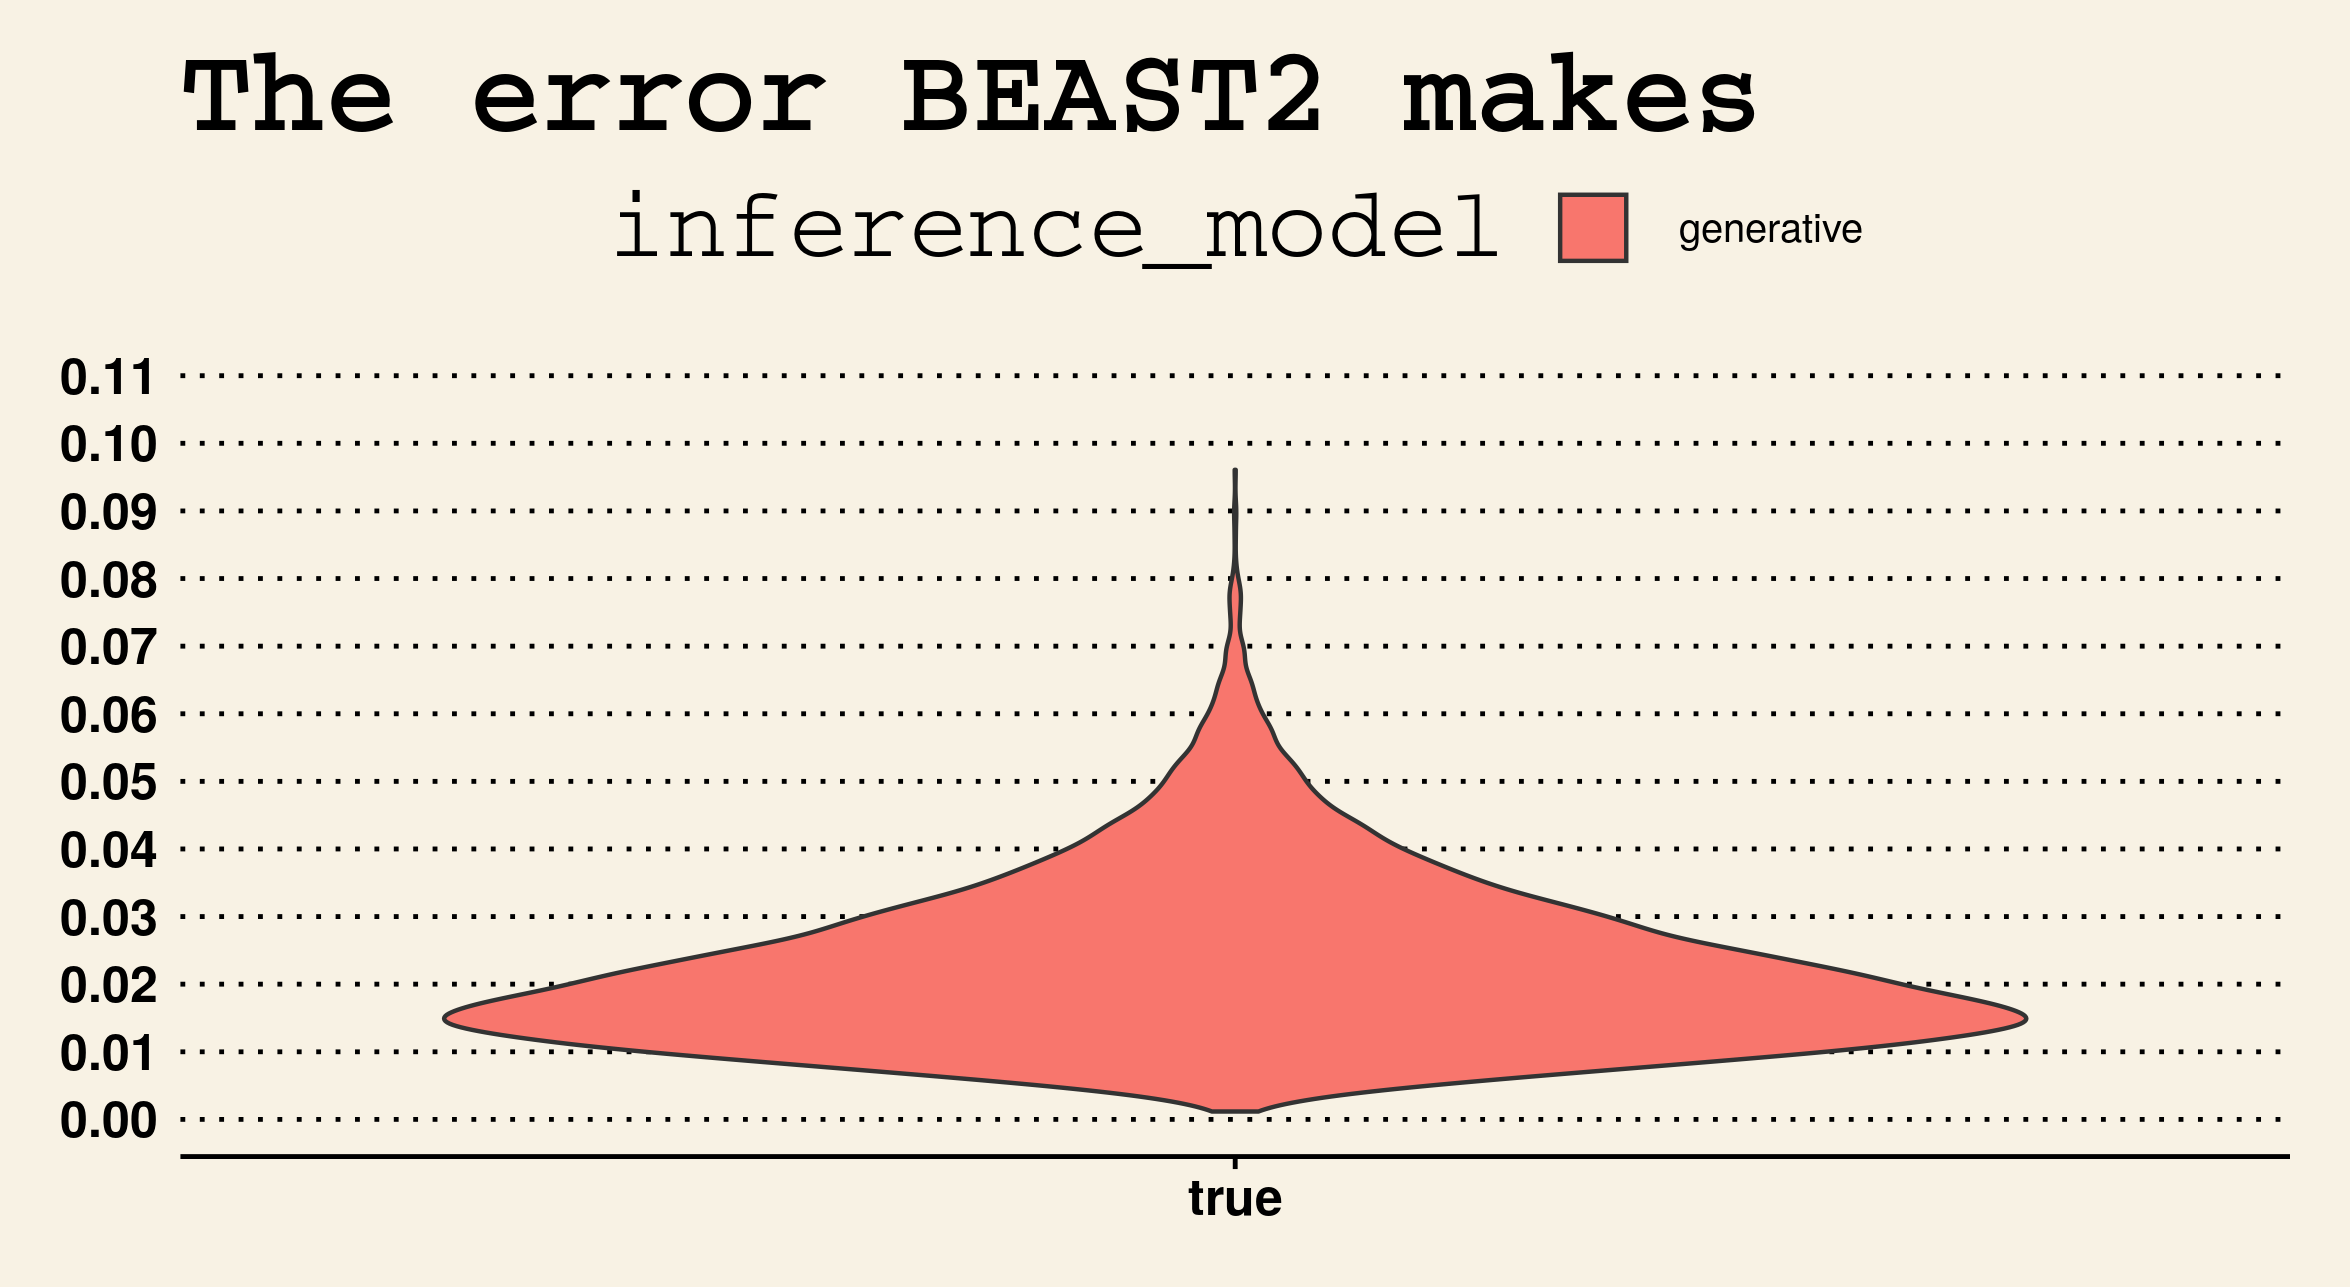
\includegraphics[width=\textwidth]{figure_example_1.png}
  \caption{
    Example 1: the error BEAST2 makes from a phylogeny 
    when the generative and inference model are the same.
    The x-axis specifies the tree type (which can be 'true' or 'twin'), 
    the y-axis shows the error. 
    The boxplot shows the minimum, first quartile, median, third 
    quartile and maximum error, of which the values are displayed 
    in the adjacent label
  }
  \label{fig:example_1}
\end{figure}

%%%%%%%%%%%%%%%%%%%%%%%%%%%%%%%%%%%%%%%%%%%%%%%%%%%%%%%%%%%%%%%%%%%%%%%%%%%%%%%%%%%%%%
\section{Usage: Example Research Question 2}
%%%%%%%%%%%%%%%%%%%%%%%%%%%%%%%%%%%%%%%%%%%%%%%%%%%%%%%%%%%%%%%%%%%%%%%%%%%%%%%%%%%%%%

A second research question that \verb;pirouette; can answer, is:

"What is the error made by BEAST2 from a phylogeny when
picking the best inference model?"

Here we start with a tree generated from an unknown 
diversification model, that has four taxa and a crown age of five:

\begin{lstlisting}[
  language=R, 
  floatplacement=H, 
  frame=single, 
  label = {lst:unknown_phylogeny},
  caption = A phylogeny generated by an unknown diversification model
]
phylogeny <- ape::read.tree(text = "((A:4, B:4):1, (C:4, D:4):1);")
\end{lstlisting}

The first step in \verb;pirouette; is to simulate a DNA alignment from the given phylogeny. 
We will re-use the alignment parameters of the previous example 
as shown in listing \ref{lst:create_alignment}.

\begin{table}
  \begin{tabular}{ | c | c | c | l | }
    \hline
    \textbf{model type} & \textbf{run if} & \textbf{measure evidence} & \textbf{inference model} \\ 
    \hline
    candidate & best candidate & yes & JC, strict, Yule \\
    candidate & best candidate & yes & JC, strict, BD   \\
    ...       & ...            & ... & ...              \\
    candidate & best candidate & yes & GTR, RLN, CCP    \\
    candidate & best candidate & yes & GTR, RLN, CEP    \\
    \hline
  \end{tabular}
  \caption{
    Experimental setup to answer the second research question.
    JC: Jukes-Cantor site model.
    strict: strict clock model.
    Yule: Yule (pure-birth) tree prior.
    BD: birth-death tree prior.
    GTR: GTR site model.
    RLN: relaxed log-normal clock model.
    CCP: coalescent constant-population tree prior.
    CEP: coalescent exponential-population tree prior.
  }
\end{table}

In the second step we state our experiments. 
Within this example, all our experiments are candidates,
run only if it is the best candidate, the evidence is measured (ignoring
this will give a helpful error) and we use the full set of 
40 inference models, which are all combinations of 4 site 
models, 2 clock models and 5 tree priors.

\begin{lstlisting}[language=R, floatplacement=H, frame=single]
experiments <- create_all_experiments()
\end{lstlisting}

Also here, the third (the BEAST2 inference) and fourth (measuring the error)
steps have sensible defaults, and we are not
interested in using a twin tree. We can create the complete
\verb;pirouette; parameter set (again) like this:

\begin{lstlisting}[language=R, floatplacement=H, frame=single]
pir_params <- create_pir_params(
  alignment_params = alignment_params,
  experiments = experiments
)
\end{lstlisting}

Running the experiment:

\begin{lstlisting}[language=R, floatplacement=H, frame=single]
errors <- pir_run(
  phylogeny,
  pir_params = pir_params
)
\end{lstlisting}

Again, showing the results:

\begin{lstlisting}[language=R, floatplacement=H, frame=single]
pir_plot(errors)
\end{lstlisting}

The resulting figure is shown in figure \ref{fig:example_2}.

\giovanni{describe winner}

\begin{figure}[h]
  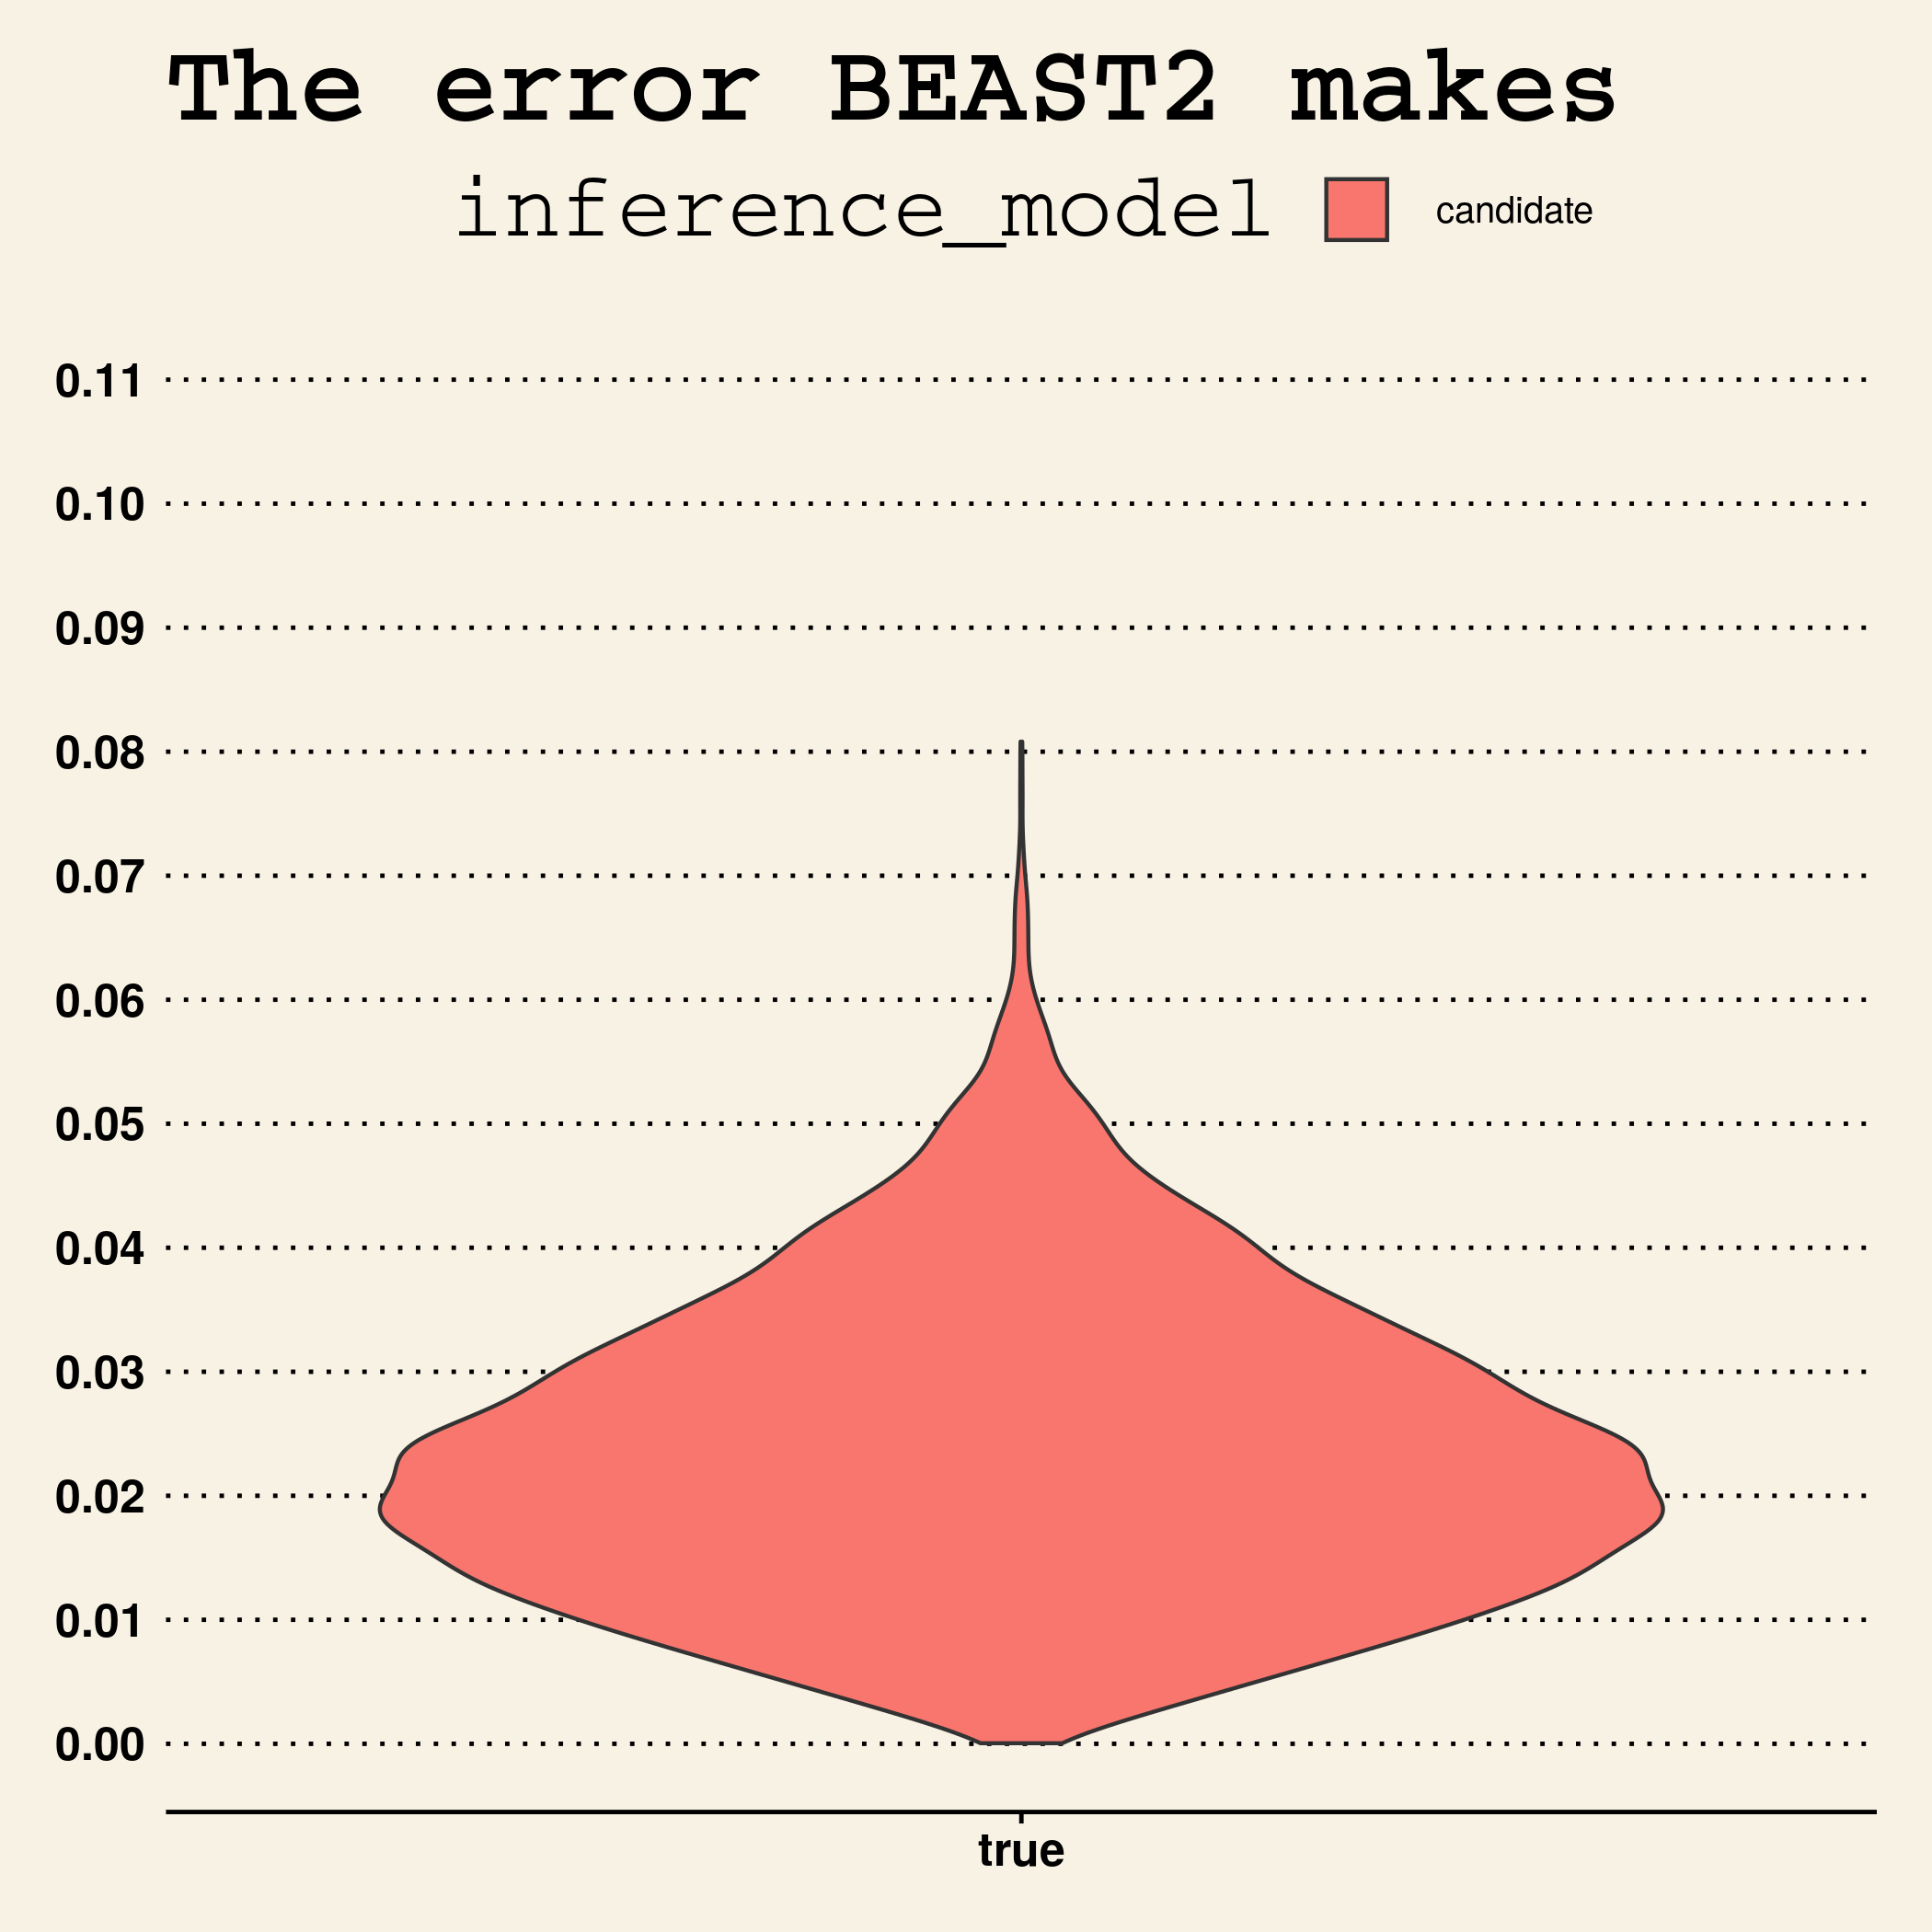
\includegraphics[width=\textwidth]{figure_example_2.png}
  \caption{
    Example 2: the error BEAST2 makes from a phylogeny when
    picking the best inference model.
    The x-axis specifies the tree type (which can be 'true' or 'twin'), the y-axis shows the error.
    The boxplot shows the minimum, first quartile, median, third 
    quartile and maximum error, of which the values are displayed 
    in the adjacent label
  }
  \label{fig:example_2}
\end{figure}

%%%%%%%%%%%%%%%%%%%%%%%%%%%%%%%%%%%%%%%%%%%%%%%%%%%%%%%%%%%%%%%%%%%%%%%%%%%%%%%%%%%%%%
\section{Usage: Example Research Question 3}
%%%%%%%%%%%%%%%%%%%%%%%%%%%%%%%%%%%%%%%%%%%%%%%%%%%%%%%%%%%%%%%%%%%%%%%%%%%%%%%%%%%%%%

A third research question that \verb;pirouette; can answer is:

"What is the error made by BEAST2 from a phylogeny, 
when hand-picking an inference model, compared to the background noise?"

The following settings are the same as in the previous section:
phylogeny (listing \ref{lst:unknown_phylogeny}), 
alignment parameters (listing \ref{lst:create_alignment}), 
experiments (listing \ref{lst:create_generative_experiment}),
BEAST2 inference and error measuring parameters \giovanni{can we add a reference to the "BEAST2 inference and error measuring parameters" we are using?}.

This time, we are interested in creating a twin tree. A twin tree
has the same topology as the given tree, 
yet its branching times are simulated according 
to the tree prior used by BEAST2 to produce a posterior. 
Since there is coherence between the inference model and the generative model, we expect BEAST2 to produce a posterior of phylogenies clearly more similar to the original one. 
We intend to use this as a control experiment.

Creating a twinning parameter is easy, as it has sensible default settings:

\begin{lstlisting}[language=R, floatplacement=H, frame=single]
twinning_params <- create_twinning_params()
\end{lstlisting}

We can now measure the errors made by BEAST2 when inferring the given phylogeny versus the error it makes when the same procedure is applied to the twin tree.

All the \verb;pirouette; arguments are bundled and checked by \verb;create_pir_params;:

\begin{lstlisting}[language=R, floatplacement=H, frame=single]
pir_params <- create_pir_params(
  alignment_params = alignment_params,
  experiments = experiments,
  twinning_params = twinning_params
)
\end{lstlisting}

Running:

\begin{lstlisting}[language=R, floatplacement=H, frame=single]
errors <- pir_run(
  phylogeny,
  pir_params = pir_params
)
\end{lstlisting}

Again, showing the results:

\begin{lstlisting}[language=R, floatplacement=H, frame=single]
pir_plot(errors)
\end{lstlisting}

The resulting figure is shown in figure \ref{fig:example_3}

\begin{figure}[h]
  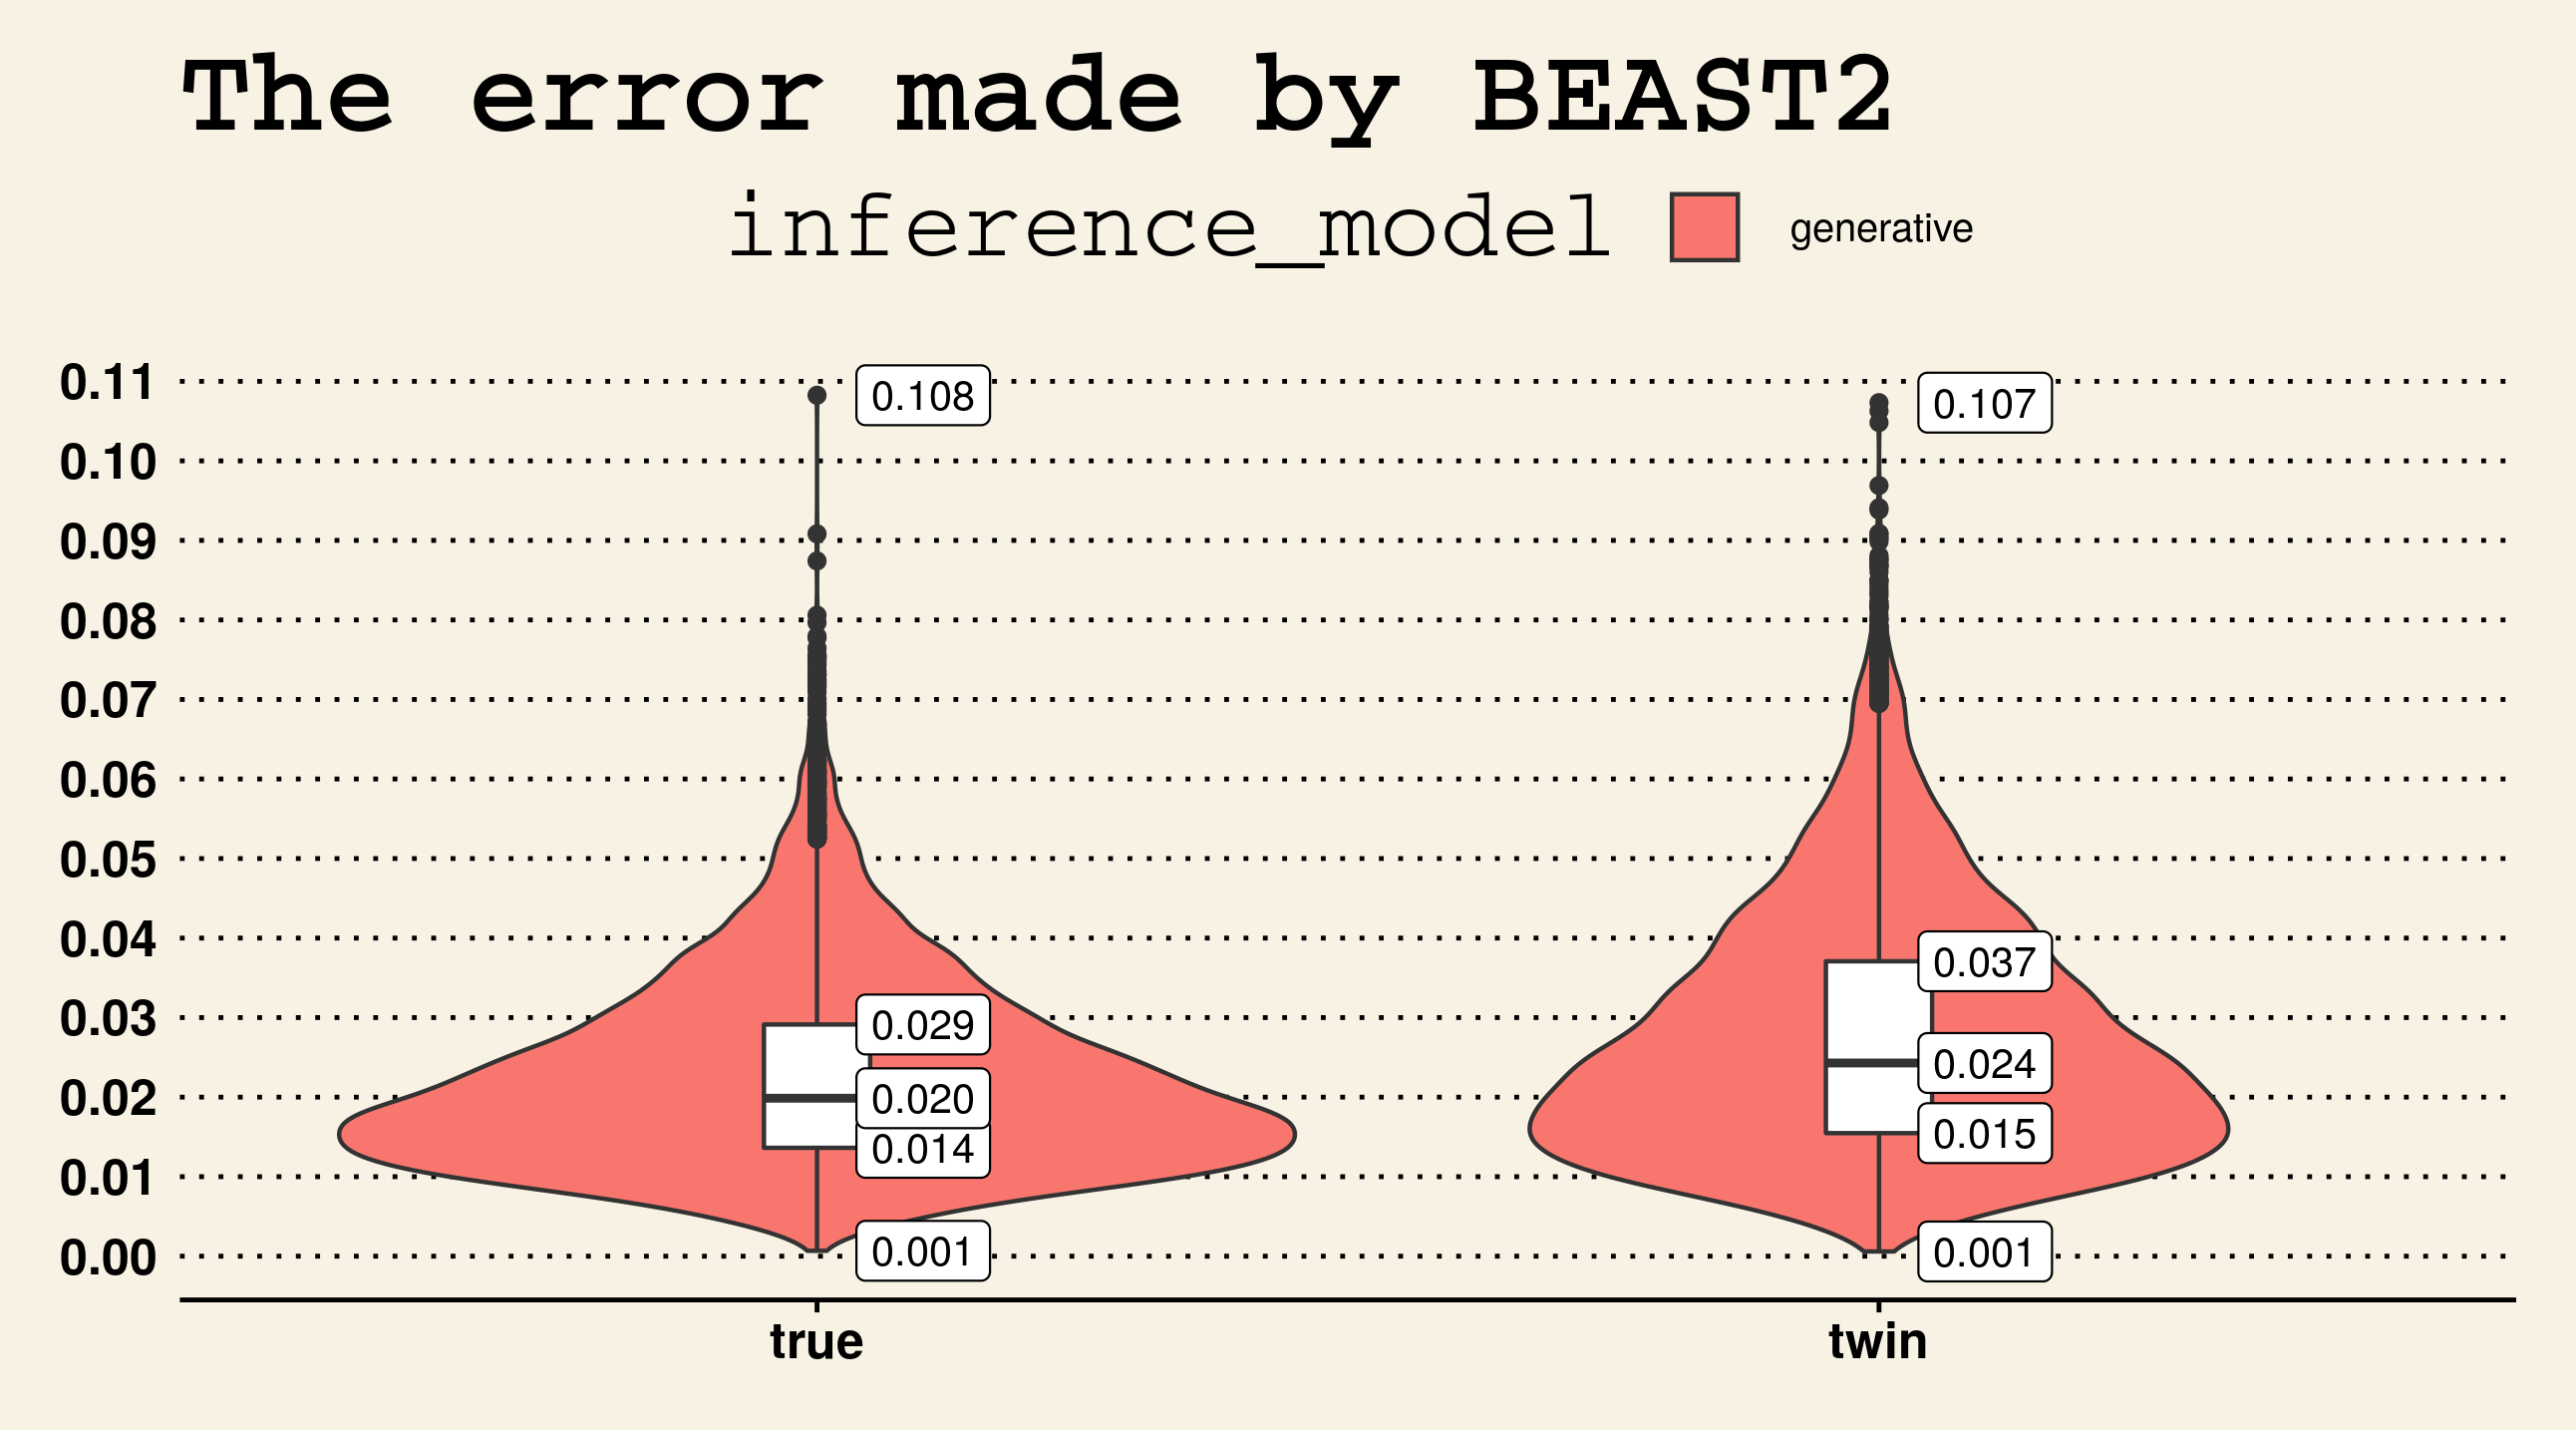
\includegraphics[width=\textwidth]{figure_example_3.png}
  \caption{
    Example 3: the error made by BEAST2 from a phylogeny, picking the best inference model versus the control.
    Here, the twin column shows the error BEAST2 makes starting from the original tree versus the twin. 
    The x-axis specifies the tree type (which can be 'true' or 'twin'), the y-axis shows the error.
    The boxplot shows the minimum, first quartile, median, third 
    quartile and maximum error, of which the values are displayed 
    in the adjacent label
  }
  \label{fig:example_3}
\end{figure}

\iffalse
The error BEAST2 makes from a phylogeny 
picking the best inference model, compared to the background noise.
Here, the twin column shows the error BEAST2 makes on an idealized
tree, to measure the noise, which is the minimal error. 
\fi


%%%%%%%%%%%%%%%%%%%%%%%%%%%%%%%%%%%%%%%%%%%%%%%%%%%%%%%%%%%%%%%%%%%%%%%%%%%%%%%%%%%%%%
\section{Usage: Example Research Question 4}
%%%%%%%%%%%%%%%%%%%%%%%%%%%%%%%%%%%%%%%%%%%%%%%%%%%%%%%%%%%%%%%%%%%%%%%%%%%%%%%%%%%%%%

A fourth research question that \verb;pirouette; can answer, is:

"What is the error made by BEAST2 from a phylogeny, when the generative model is known, compared to candidates with similar inference models, in relationship to the background error?"

Here, same as example 2, we start with a tree generated by the Yule process, by using the code shown in listing \ref{lst:create_yule_tree}.
The first step in \verb;pirouette; is to simulate a DNA alignment 
from the given phylogeny, for which we will use the same code 
as shown in listing \ref{lst:create_alignment}.

\begin{table}
  \begin{tabular}{ | c | c | c | l | }
    \hline
    \textbf{model type} & \textbf{run if} & \textbf{measure evidence} & \textbf{inference model} \\ 
    \hline
    generative & always         & yes & JC, strict, Yule \\
    candidate  & best candidate & yes & JC, strict, BD \\
    candidate  & best candidate & yes & JC, strict, CCP \\
    candidate  & best candidate & yes & JC, strict, CEP \\
    \hline
  \end{tabular}
  \caption{
    Experimental setup to answer the fourth research question.
    JC: Jukes-Cantor site model.
    strict: strict clock model.
    Yule: Yule (pure-birth) tree prior.
    BD: birth-death tree prior.
    CCP: coalescent constant-population tree prior.
    CEP: coalescent exponential-population tree prior.
  }
  \label{tab:experiment_4}
\end{table}

In the second step we state our experiments. 
In this example, we must both specify the generative and candidate experiments. Here we specify the generative model:

\begin{lstlisting}[language=R, floatplacement=H, frame=single]
generative_experiment <- create_experiment(
  model_type = "generative",
  run_if = "always",
  do_measure_evidence = TRUE
)
\end{lstlisting}

Specifying all candidates can be done simply by calling \verb;create_all_experiments;. In this case, all candidates will use the same site and clock model, and only differ in their tree priors:

\begin{lstlisting}[language=R, floatplacement=H, frame=single]
candidate_experiments <- create_all_experiments(
  site_models = list(create_jc69_site_model()),
  clock_models = list(create_strict_clock_model()),
  tree_priors = list(
    create_bd_tree_prior(), 
    create_ccp_tree_prior(), 
    create_cep_tree_prior()
  )
)
\end{lstlisting}

We need to combine these experiments into one set:

\begin{lstlisting}[language=R, floatplacement=H, frame=single]
experiments <- c(list(generative_experiment), candidate_experiments)
\end{lstlisting}

We choose again to use sensible defaults for the third (the BEAST2 inference) and fourth (measuring the error) steps, as we previously did to answer the second research question. To get an idea of a baseline error made by BEAST2, we also make use of the twinning option:

\begin{lstlisting}[language=R, floatplacement=H, frame=single]
pir_params <- create_pir_params(
  alignment_params = alignment_params,
  experiments = experiments,
  twinning_params = create_twinning_params()
)
\end{lstlisting}

Running the experiment:

\begin{lstlisting}[language=R, floatplacement=H, frame=single]
errors <- pir_run(
  phylogeny,
  pir_params = pir_params
)
\end{lstlisting}

Again, showing the results:

\begin{lstlisting}[language=R, floatplacement=H, frame=single]
pir_plot(errors)
\end{lstlisting}

The resulting figure is shown in figure \ref{fig:example_4}.

\giovanni{describe winner}

\begin{figure}[h]
  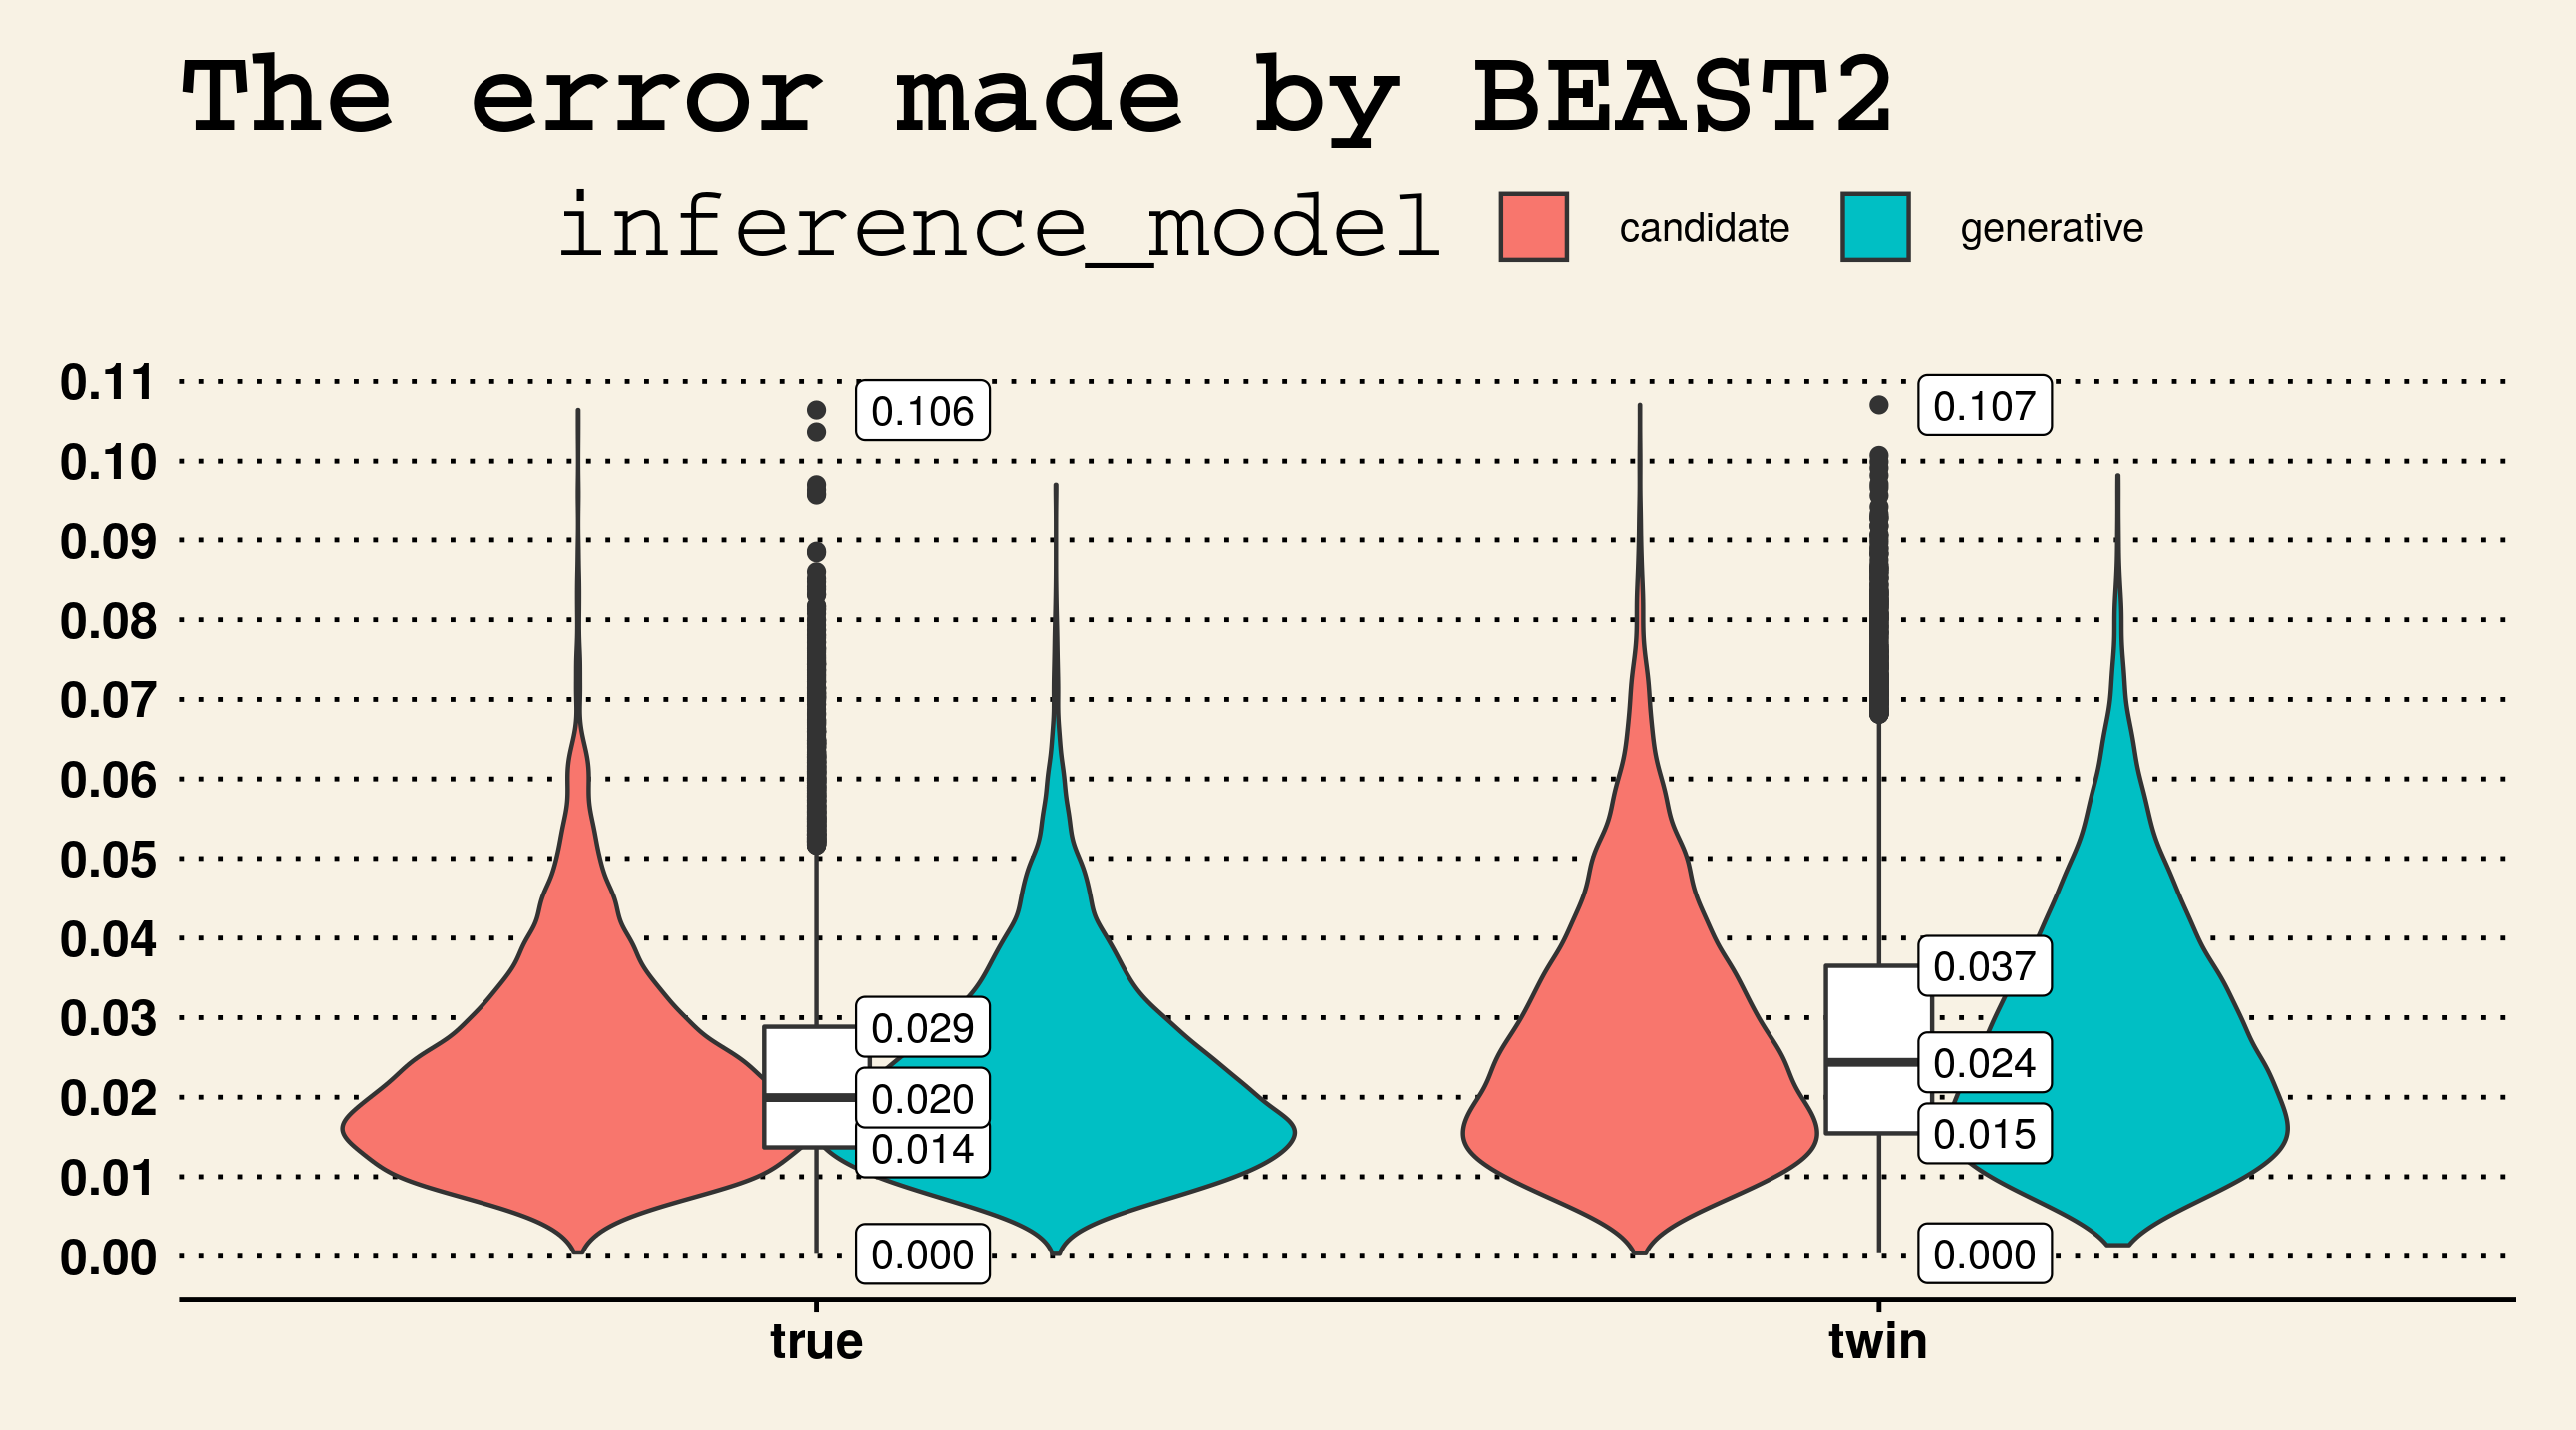
\includegraphics[width=\textwidth]{figure_example_4.png}
  \caption{
    Example 4: the error made by BEAST2 from a phylogeny, when the generative model is known, compared to candidates with similar inference models, in relationship to the background error.
    The x-axis specifies the tree type, the y-axis shows the error.
    The boxplot shows the minimum, first quartile, median, third 
    quartile and maximum error, of which the values are displayed 
    in the adjacent label
  }
  \label{fig:example_4}
\end{figure}

%%%%%%%%%%%%%%%%%%%%%%%%%%%%%%%%%%%%%%%%%%%%%%%%%%%%%%%%%%%%%%%%%%%%%%%%%%%%%%%%%%%%%%
\section{Discussion}
%%%%%%%%%%%%%%%%%%%%%%%%%%%%%%%%%%%%%%%%%%%%%%%%%%%%%%%%%%%%%%%%%%%%%%%%%%%%%%%%%%%%%%

%%%%%%%%%%%%%%%%%%%%%%%%%%%%%%%%%%%%%%%%%%%%%%%%%%%%%%%%%%%%%%%%%%%%%%%%%%%%%%%%%%%%%%
\begin{table}[h]
\centering
\begin{tabular}{ | r | l | l | l | l | }
\hline
\multirow{2}{*}{\textbf{Example}} & \multicolumn{2}{c|}{\textbf{True tree}} 
                                  & \multicolumn{2}{c|}{\textbf{Twin tree}} \\
\cline{2-5}
                                  & \textbf{median} & \textbf{range} & \textbf{median} & \textbf{range} \\
\hline
1  & $0.02$  & $0.0 - 0.27$  &         &               \\
2  & $0.02$  & $0.0 - 0.08$  &         &               \\
3  & $0.018$ & $0.0 - 0.1$   & $0.019$ & $0.0 - 0.11$  \\
4C & $0.22$  & $0.0 - 0.088$ & $0.009$ & $0.0 - 0.056$ \\
4G & $0.020$ & $0.0 - 0.075$ & $0.013$ & $0.0 - 0.052$ \\
\hline
\end{tabular}
\caption{Results of the examples. 
  For the true and twin tree,
  the median and range (from minimum to maximum value) of the errors 
  is shown. Experiment 4 is split in two rows
  by either the candidate ('C') or generative model ('G')
}
\label{tab:results}
\end{table}
%%%%%%%%%%%%%%%%%%%%%%%%%%%%%%%%%%%%%%%%%%%%%%%%%%%%%%%%%%%%%%%%%%%%%%%%%%%%%%%%%%%%%%

\richel{check numbers}
\giovanni{I think that the current version of the discussion is too didascalic. Most of what is said can be effectively summarized by table 5. We can even add ESSes in it. Another point is that we should understand what is the message we want to deliver in this discussion. Since we are only using one tree we are not in the position to claim anything, because a single tree is not an effective sample. I saw that in some occasions you refer to the RQ as examples. This might be the right way to proceed, as our purpose is just to illustrate how to run all the possible experiments on a full tree distribution. I think we should make it clearer throughout the entire manuscript. I am also interested in hearing Rampal's opinion on this.}

\iffalse
Here we discuss how to interpret the results of \verb;pirouette;.
Figure \ref{fig:example_1} shows that the generative model 
gives an error distribution with a median of \richel{?}
The range of errors goes from \richel{?} to \richel{?}.
As we know the generative model, this error distribution is the minimum noise that BEAST2 produces for that generative model.
We can measure the effective samples as well (not shown), 
and all the Estimated Sample Sizes (ESSes) are above
the recommended value of 200 [\cite{drummond2015bayesian}], 
as shown in table \ref{tab:esses_example_1}.

Figure \ref{fig:example_2} shows that the best candidate model gives an error distribution with a median of \richel{?}. 
The range of errors goes from \richel{?} to \richel{?}. 
The inference model with the highest evidence follows a JC site model, RLN clock model and BD tree prior, with a weight of $0.675$. 
This is (unexpectedly) \giovanni{We are not using distributions, so we are totally subject to stochasticity. Nothing can be expected from just one tree.} better than the generative
model with a weight of $0.166$. 
The complete list of all evidences is shown in table \ref{tab:evidences_example_2}.
This means that it is rational to use this inference model to 
infer a posterior phylogeny distribution, as is done by \verb;pirouette;.
Also here, the ESSes are well above 200, 
as shown in table \ref{tab:esses_example_2}.

Figure \ref{fig:example_3} shows that the hand-picked model 
gives an error distribution with a median of \richel{?}, 
The twin tree has an error distribution with a median of \richel{?},
with a range from 0.0 to \richel{?}, which is an indication of the
error made by BEAST on that tree prior.
As there is little difference between the true and twin tree,
the (unknown) diversification model has little impact on the error
BEAST2 makes, hinting that the constant-rate birth-death model is
sufficiently good enough to explain the true phylogeny. 
The diversification model apparently has minor impact and need not to be
added to BEAST2.
We can draw this conclusion with confidence, as the ESSes are well above 200, 
as shown in table \ref{tab:esses_example_3}.

Figure \ref{fig:example_4} shows that \richel{?}
and 
gives an error distribution with a median of \richel{?}, 
The twin tree has an error distribution with a median of \richel{?},
with a range from 0.0 to \richel{?}, which is an indication of the
error made by BEAST on that tree prior.
The inference model with the highest evidence follows a JC site model, 
RLN clock model and BD tree prior, with a weight of ?. 
The complete list of all evidences is shown in table \ref{tab:evidences_example_4}.
As there is little difference between the true and twin tree,
the (unknown) diversification model has little impact on the error
BEAST2 makes, hinting that the constant-rate birth-death model is
sufficiently good enough to explain the true phylogeny. 
The diversification model apparently has minor impact and need not to be
added to BEAST2.
We can draw this conclusion with confidence \giovanni{no, we cannot: one tree is not enough}, as the ESSes are well above 200, 
as shown in table \ref{tab:esses_example_4}.
\fi

\giovanni{This is a first draft on how I think the discussion should be setup. In this context there is no much need for the results in the table. Let me know what you think about it.}

In the four example research questions we showed how to use \verb;pirouette; to assess if BEAST2 is able, with a birth-death prior, to recover the original tree simulated by a Yule process. In principle any other, possibly much more complex, generative prior can be tested.
All tests were performed on a single original tree, hence not providing us enough statistical power to evaluate the level of accuracy of the inference. However if the same procedure were repeated and performed on a distribution with a sufficient number of generative trees, it could actually constitute a quantitative assessment of the quality of the inference, as shown in figures \ref{fig:example_1}, \ref{fig:example_2}, \ref{fig:example_3}, \ref{fig:example_4}. Importantly, \verb;pirouette; can directly show the comparison between the results obtained on a new generative prior as compared to the error BEAST2 would make when operating on a tree generated under the right tree prior (the twin tree).
From such results an user can estimate whether or not a new tree prior, tailored on the generative process, is needed. If this would indeed be the case, one could implement their own tree prior as a new module in BEAST2.
\giovanni{Maybe we can add a bit more on the nested sampling.}

%%%%%%%%%%%%%%%%%%%%%%%%%%%%%%%%%%%%%%%%%%%%%%%%%%%%%%%%%%%%%%%%%%%%%%%%%%%%%%%%%%%%%%
\section{pirouette resources}
%%%%%%%%%%%%%%%%%%%%%%%%%%%%%%%%%%%%%%%%%%%%%%%%%%%%%%%%%%%%%%%%%%%%%%%%%%%%%%%%%%%%%%

\verb;pirouette; is free, libre and open source software available at 
\url{http://github.com/richelbilderbeek/pirouette}
and is licensed under the GNU General Public License v3.0.
\verb;pirouette; follows all practices as recommended by the
literature: continuous integration, a code coverage of 100\%
and a style guide (\cite{style_guide}).
\verb;pirouette; depends on multiple packages, which are 
\verb;ape; (\cite{APE}), 
\verb;babette; (\cite{bilderbeek2018babette}),
\verb;ggplot2; (\cite{ggplot2}),
\verb;knitr; (\cite{knitr}),
\verb;mcbette; (\cite{mcbette}),
\verb;phangorn; (\cite{phangorn}),
\verb;rmarkdown; (\cite{rmarkdown}),
\verb;stringr; (\cite{stringr}),
\verb;testit; (\cite{testit}) and 
\verb;usethis; (\cite{usethis}).

\verb;pirouette;'s development takes place on GitHub,
\url{https://github.com/richelbilderbeek/pirouette}, 
which facilitates feature requests and 
has guidelines on how to do so.

\verb;pirouette;'s documentation is extensive. All functions are documented in the package's internal documentation. For quick use, 
each exported function shows a minimal example. 
For easy exploration, each exported function's documentation links to related functions.
Additionally, \verb;pirouette; has a vignette that demonstrates extensively how to use it. 

%%%%%%%%%%%%%%%%%%%%%%%%%%%%%%%%%%%%%%%%%%%%%%%%%%%%%%%%%%%%%%%%%%%%%%%%%%%%%%%%%%%%%%
\section{Citation of pirouette}
%%%%%%%%%%%%%%%%%%%%%%%%%%%%%%%%%%%%%%%%%%%%%%%%%%%%%%%%%%%%%%%%%%%%%%%%%%%%%%%%%%%%%%

Scientists using \verb;pirouette; in a published paper can cite this
article, and/or cite the \verb;pirouette; package 
directly. To obtain this citation from within an R script, use:

\begin{lstlisting}[language=R]
> citation("pirouette")
\end{lstlisting}

%%%%%%%%%%%%%%%%%%%%%%%%%%%%%%%%%%%%%%%%%%%%%%%%%%%%%%%%%%%%%%%%%%%%%%%%%%%%%%%%%%%%%%
\section{Acknowledgements}
%%%%%%%%%%%%%%%%%%%%%%%%%%%%%%%%%%%%%%%%%%%%%%%%%%%%%%%%%%%%%%%%%%%%%%%%%%%%%%%%%%%%%%

We would like to thank the Center for Information Technology of the University 
of Groningen for their support and for providing access to the Peregrine 
high performance computing cluster. 
We thank the Netherlands 
Organization for Scientific Research (NWO) for financial support 
through a VICI grant awarded to RSE.

%%%%%%%%%%%%%%%%%%%%%%%%%%%%%%%%%%%%%%%%%%%%%%%%%%%%%%%%%%%%%%%%%%%%%%%%%%%%%%%%%%%%%%
\section{Data Accessibility}
%%%%%%%%%%%%%%%%%%%%%%%%%%%%%%%%%%%%%%%%%%%%%%%%%%%%%%%%%%%%%%%%%%%%%%%%%%%%%%%%%%%%%%

All code is archived at \url{http://github.com/richelbilderbeek/pirouette_article},
with DOI \url{https://doi.org/12.3456/zenodo.1234567}.

%%%%%%%%%%%%%%%%%%%%%%%%%%%%%%%%%%%%%%%%%%%%%%%%%%%%%%%%%%%%%%%%%%%%%%%%%%%%%%%%%%%%%%
\section{Authors' contributions}
%%%%%%%%%%%%%%%%%%%%%%%%%%%%%%%%%%%%%%%%%%%%%%%%%%%%%%%%%%%%%%%%%%%%%%%%%%%%%%%%%%%%%%

RJCB, GL and RSE conceived the idea for the package. 
RJCB created and tested the package, and wrote the first draft of the manuscript.
GL tested the package and contributed substantially to revisions.
RSE contributed to revisions.

%%%%%%%%%%%%%%%%%%%%%%%%%%%%%%%%%%%%%%%%%%%%%%%%%%%%%%%%%%%%%%%%%%%%%%%%%%%%%%%%%%%%%%
% Bibliography
%%%%%%%%%%%%%%%%%%%%%%%%%%%%%%%%%%%%%%%%%%%%%%%%%%%%%%%%%%%%%%%%%%%%%%%%%%%%%%%%%%%%%%
% MEE style
\bibliographystyle{mee}
\bibliography{article}
%%%%%%%%%%%%%%%%%%%%%%%%%%%%%%%%%%%%%%%%%%%%%%%%%%%%%%%%%%%%%%%%%%%%%%%%%%%%%%%%%%%%%%

\appendix

%%%%%%%%%%%%%%%%%%%%%%%%%%%%%%%%%%%%%%%%%%%%%%%%%%%%%%%%%%%%%%%%%%%%%%%%%%%%%%%%%%%%%%
\section{Results in detail}
%%%%%%%%%%%%%%%%%%%%%%%%%%%%%%%%%%%%%%%%%%%%%%%%%%%%%%%%%%%%%%%%%%%%%%%%%%%%%%%%%%%%%%

\richel{
  I'd enjoy to put all intermediate output here: alignments, twin trees,
  posteriors, nLTTs, errors. Now we only show the ones relevant in the text
}

\input{example_1_esses.latex}
% has label tab:esses_example_1

\input{example_2_esses.latex}
% has label tab:esses_example_2

\input{example_2_evidences.latex}
% has label tab:evidences_example_2

\input{example_3_esses.latex}
% has label tab:esses_example_3

\input{example_4_esses.latex}
% has label tab:esses_example_4

\input{example_4_evidences.latex}
% has label tab:evidences_example_4

\end{document}
